% LaTeX document skeleton
% generated on Tue Jan 04 15:00:38 +0100 2011
% by Kévin Fardel et Rick Ghanem
% With the Condom lib (version 1.1.0)
% See http://github.com/v0n/condom

%%%%%%%%%%%%%
% PREAMBULE %
%%%%%%%%%%%%%

\documentclass[a4paper, 11pt]{article}           % format general

% LaTeX packages to import
% generated on Tue Jan 04 15:00:38 +0100 2011
% by Kévin Fardel et Rick Ghanem
% With the Condom lib (version 1.1.0)
% See http://github.com/v0n/condom

\usepackage[T1]{fontenc}      % codage des caracteres

\usepackage[utf8]{inputenc}   % encodage du fichier (utf8 ou latin1)
\usepackage[francais]{babel}  % langue
\usepackage{mathpazo}         % selection de la police
\usepackage{geometry}         % mise en page
\usepackage{xcolor}           % pour colorer des elements

\usepackage{graphicx}         % pour inserer des images

% math
\usepackage{amssymb}          % symboles mathematiques
%\usepackage{amsmath}         % commandes mathematiques

% pdf
\usepackage{url}              % permet l'insertion d'url
\usepackage[pdftex]{hyperref} % permet l'hypertexte (rend les liens cliquables)

% listings
\usepackage{listings}         % permet d'inserer du code (multi-langage)
\usepackage{courier}
\usepackage{caption}

% fancyhdr
\usepackage{lastpage}         % derniere page
\usepackage{fancyhdr}         % en-tete et pied de page

\usepackage{multicol}


% Customized colors
% generated on Tue Jan 04 15:00:38 +0100 2011
% by Kévin Fardel et Rick Ghanem
% With the Condom lib (version 1.1.0)
% See http://github.com/v0n/condom

%         Colors    Bright Colors
% Black   #0F2130   #B0B3B9
% Red     #D22613   #F96795
% Green   #7CDE53   #A0F2A0
% Yellow  #EBE645   #F4EF82
% Blue    #2C9ADE   #A3FEFE
% Orange  #FFA705   #F1B356
% Cyan    #8A95A7   #B0C3DA
% White   #F8F8F8   #FFFFFF

\definecolor{myblack}{HTML}{0F2130}
\definecolor{myred}{HTML}{D22613}
\definecolor{mygreen}{HTML}{7CDE53}
\definecolor{myyellow}{HTML}{EBE645}
\definecolor{myblue}{HTML}{2C9ADE}
\definecolor{myorange}{HTML}{FFA705}
\definecolor{mycyan}{HTML}{8A95A7}
\definecolor{mywhite}{HTML}{F8F8F8}
\definecolor{mygrey}{HTML}{555753}

% Personal commands
% generated on Tue Jan 04 15:00:38 +0100 2011
% by Kévin Fardel et Rick Ghanem
% With the Condom lib (version 1.1.0)
% See http://github.com/v0n/condom

% raccourcis
\newcommand{\Cad}{C'est-à-dire~}
\newcommand{\cad}{c'est-à-dire~}
\newcommand{\pe}{peut-être~}

\newcommand{\todo}[1]{\bigskip \colorbox{myyellow}{\textcolor{mygrey}{\textsf{\textbf{TODO} #1 }}} \bigskip}

\newcommand{\name}[2]{#1 \textsc{#2}}

\newcommand{\email}[1]{\href{mailto:#1}{\textsf{<#1>}}}

% commande pour afficher un lien vers une image
\newcommand{\figref}[1]{\textsc{Fig.}~\ref{#1} (p.~\pageref{#1})}

% commande pour afficher le lien vers un listing :
\newcommand{\lstref}[1]{{\footnotesize Listing~\ref{#1}, p.~\pageref{#1}}}



% listings package config file
% generated on Tue Jan 04 15:00:38 +0100 2011
% by Kévin Fardel et Rick Ghanem
% With the Condom lib (version 1.1.0)
% See http://github.com/v0n/condom

% /!\ ne pas utiliser de caracteres accentues dans les sources (ne gere pas l'utf-8)
% pour remplacer les lettres accentues : sed -i -e "y/ÉÈÊÇÀÔéèçàôîêûùï/EEECAOeecaoieuui/" fichier

% configuration des listings par defaut :
\lstset{
    basicstyle=\footnotesize\ttfamily,
    %numbers=left,
    numberstyle=\tiny,
    %stepnumber=2,
    numbersep=5pt,
    tabsize=2,
    extendedchars=true,
    breaklines=true,
    frame=b,
    keywordstyle=\color{red},
    %keywordstyle=[1]\textbf,
    %keywordstyle=[2]\textbf,
    %keywordstyle=[3]\textbf,
    %keywordstyle=[4]\textbf,
    stringstyle=\color{white}\ttfamily,
    showspaces=false,
    showtabs=false,
    xleftmargin=17pt,
    framexleftmargin=17pt,
    framexrightmargin=5pt,
    framexbottommargin=4pt,
    %backgroundcolor=\color{lightgray},
    showstringspaces=false
}

\lstloadlanguages{
    %[Visual]Basic
    %Pascal
    %C
    %C++
    %XML
    %HTML
    %Java
}
%\DeclareCaptionFont{blue}{\color{blue}}

%\captionsetup[lstlisting]{singlelinecheck=false, labelfont={blue}, textfont={blue}}
\DeclareCaptionFont{white}{\color{white}}
\DeclareCaptionFormat{listing}{\colorbox[cmyk]{0.43, 0.35, 0.35,0.01}{\parbox{\textwidth}{\hspace{15pt}#1#2#3}}}
\captionsetup[lstlisting]{format=listing,labelfont=white,textfont=white, singlelinecheck=false, margin=0pt, font={bf,footnotesize}}

% configuration des listings C :
\lstnewenvironment{C}
{\lstset{%
    language=C,
    tabsize=3,
    xleftmargin=0.75cm,
    numbers=left,
    numberstyle=\tiny,
    extendedchars=true,
    %frame=single,
    %frameround=tttt,
    framexleftmargin=8mm,
    float,
    showstringspaces=true,
    showspaces=false,
    showtabs=false,
    breaklines=true,
    backgroundcolor=\color{mywhite},
    basicstyle=\color{myblack} \small,
    keywordstyle=\color{myred} \bfseries,
    ndkeywordstyle=\color{myred} \bfseries,
    commentstyle=\color{myblue} \itshape,
    identifierstyle=\color{myyellow},
    stringstyle=\color{mygreen}
}}
{}

% configuration des listings console :
\lstnewenvironment{console}
{\lstset{%
    language={},
    numbers=none,
    extendedchars=true,
    framexleftmargin=5mm,
    %float,
    showstringspaces=false,
    showspaces=false,
    showtabs=false,
    breaklines=false,
    backgroundcolor=\color{darkgray},
    basicstyle=\color{white} \scriptsize \ttfamily,
    keywordstyle=\color{white},
    ndkeywordstyle=\color{white},
    commentstyle=\color{white},
    identifierstyle=\color{white},
    stringstyle=\color{white}
}}
{}

\renewcommand{\lstlistlistingname}{Table des codes sources} % renommer la liste des listings

% un listing depuis un fichier s'importe comme ceci :
%\lstinputlisting[caption={Legende}, label=lst:label]{emplacement}

                        % fichier de config du paquet listings

\geometry{top=2.5cm, bottom=2.5cm, left=2cm, right=2cm}

\graphicspath{{fig/}}                 % chemins vers les images

% informations du document
\author{Kévin Fardel et Rick Ghanem}
\date{\today}
\title{Rapport de Traitement du signal}

\hypersetup{%
    pdftitle    = {Rapport de Traitement du signal},
    pdfauthor   = {Kévin Fardel et Rick Ghanem}
    pdfcreator  = {Texlive},
    pdfproducer = {Texlive},
    colorlinks  = true,
    linkcolor   = black,
    citecolor   = black,
    urlcolor    = black
}                                                   % informations du pdf

\pagestyle{fancy}
\lhead{Rapport de Traitement du signal}
\chead{}
\rhead{\thepage/\pageref{LastPage}}
\lfoot{}
\cfoot{}
\rfoot{\footnotesize Kévin Fardel et Rick Ghanem}
%\renewcommand{\headrulewidth}{0pt}
%\renewcommand{\footrulewidth}{0.4pt}
\fancypagestyle{plain}{%                        % style des pages de titres
    \fancyhf{}
    \renewcommand{\headrulewidth}{0pt}
    \renewcommand{\footrulewidth}{0pt}
}

\makeatletter
\@addtoreset{section}{part} % reprendre a partir de 1 les sections des parties suivantes
\makeatother

%\AtBeginDocument{%
%   \renewcommand{\abstractname}{} % renommer le resume
%}

%%%%%%%%%
% CORPS %
%%%%%%%%%

\begin{document} % debut du document

\maketitle % afficher le titre

% resume
\begin{abstract}
\end{abstract}

\tableofcontents % table des matieres

\lstlistoflistings % tables des listings

\newpage
\part{Exercice 1}
La figure suivante nous montre la porte sur l'intervalle [-32 32] : 
\begin{figure}[H]
\centering
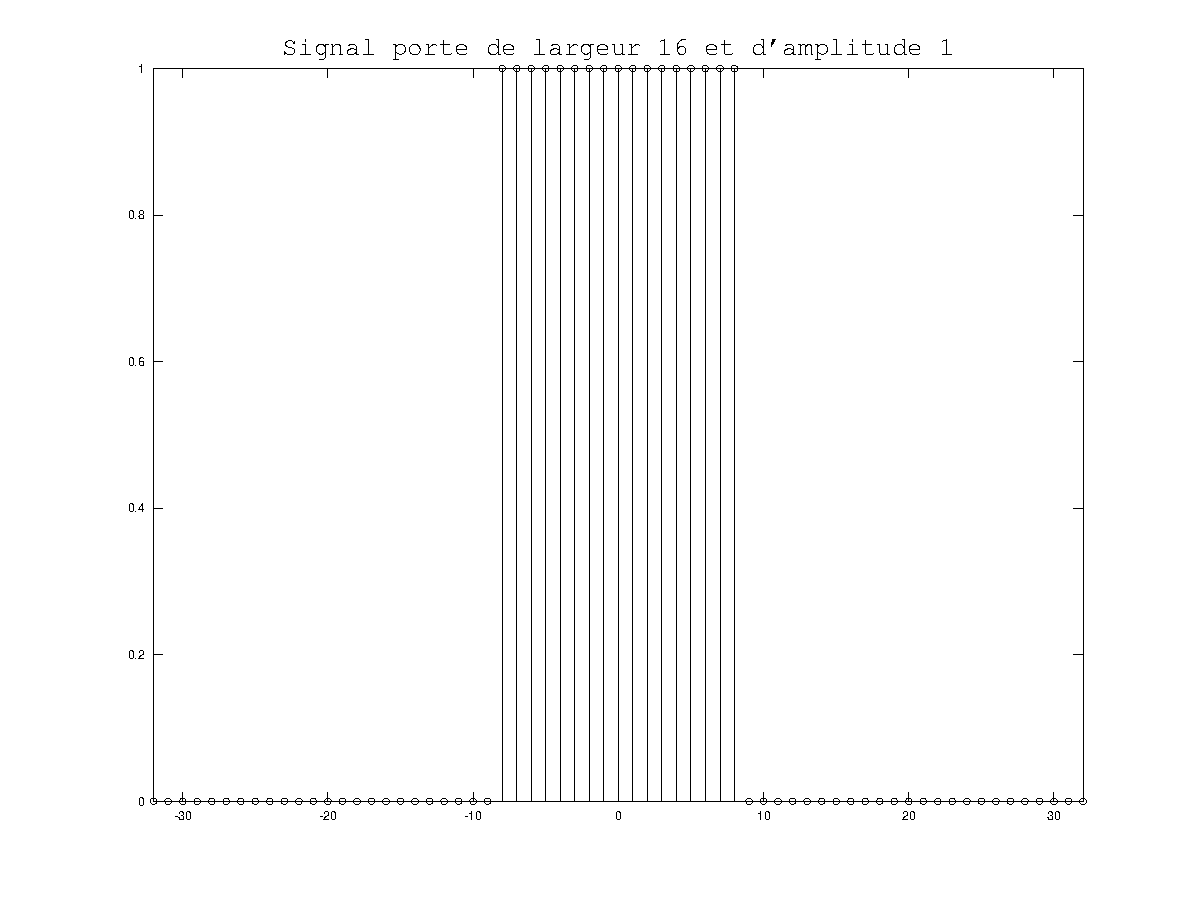
\includegraphics[width=9cm]{resEx1/signalPorte.pdf}
\caption{Signal porte sur l'intervalle [-32 32]}
\end{figure}

La transformé de Fourier de la porte sur l'intervalle [0 0.5] en fréquence réduite donne la courbe ci dessous : 
\begin{figure}[H]
\centering
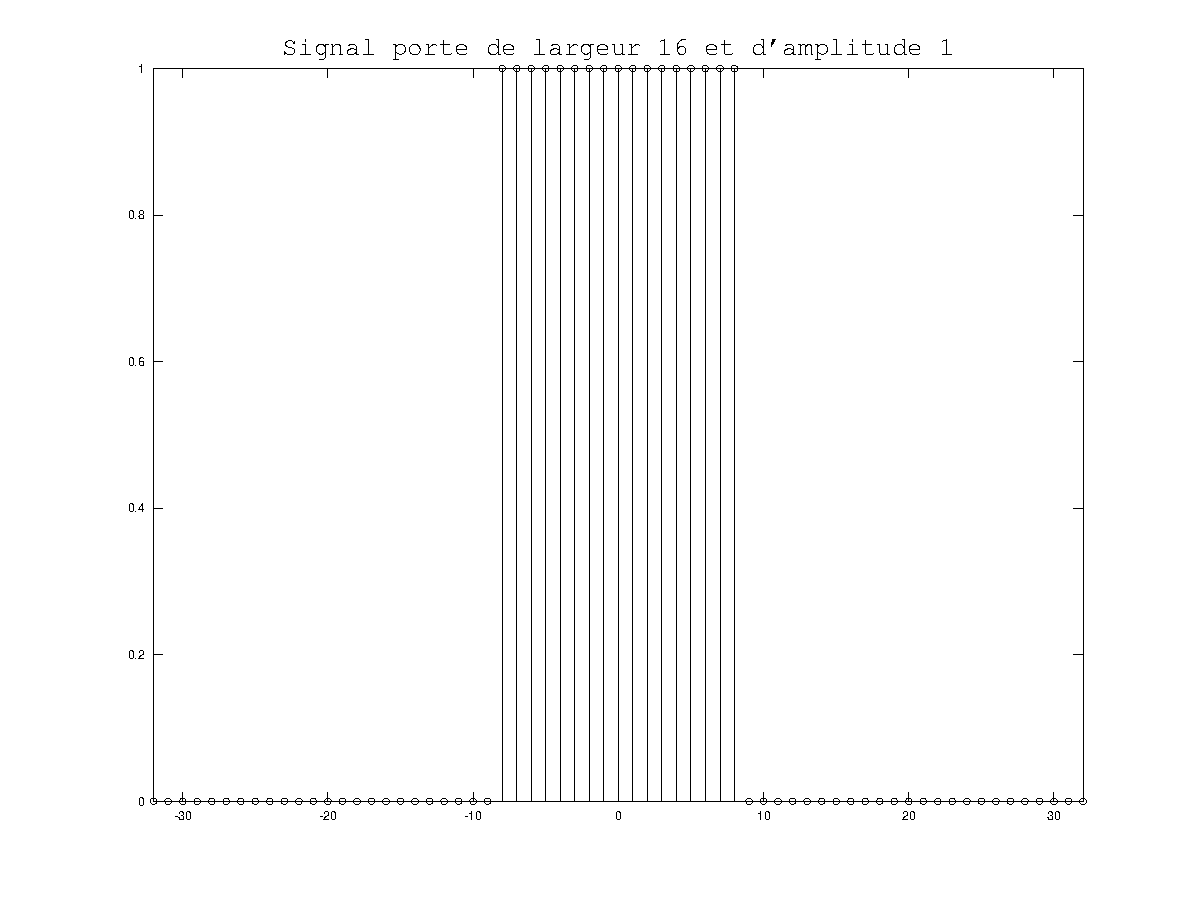
\includegraphics[width=9cm]{resEx1/signalPorte.pdf}
\caption{Signal porte sur l'intervalle [-32 32]}
\end{figure}



\part{Exercice 2}
Dans cette exercice nous faisons appel à une fonction annexe pour récupérer la fonction échelon.

Cette fonction prend en paramètre le vecteur représentant l'intervalle de visualisation ainsi que le décalage que l'on souhaite appliquer à l'échelon.

La courbe ci dessous nous illustre le filtre discret que nous avons à disposition :

\begin{figure}[H]
\centering
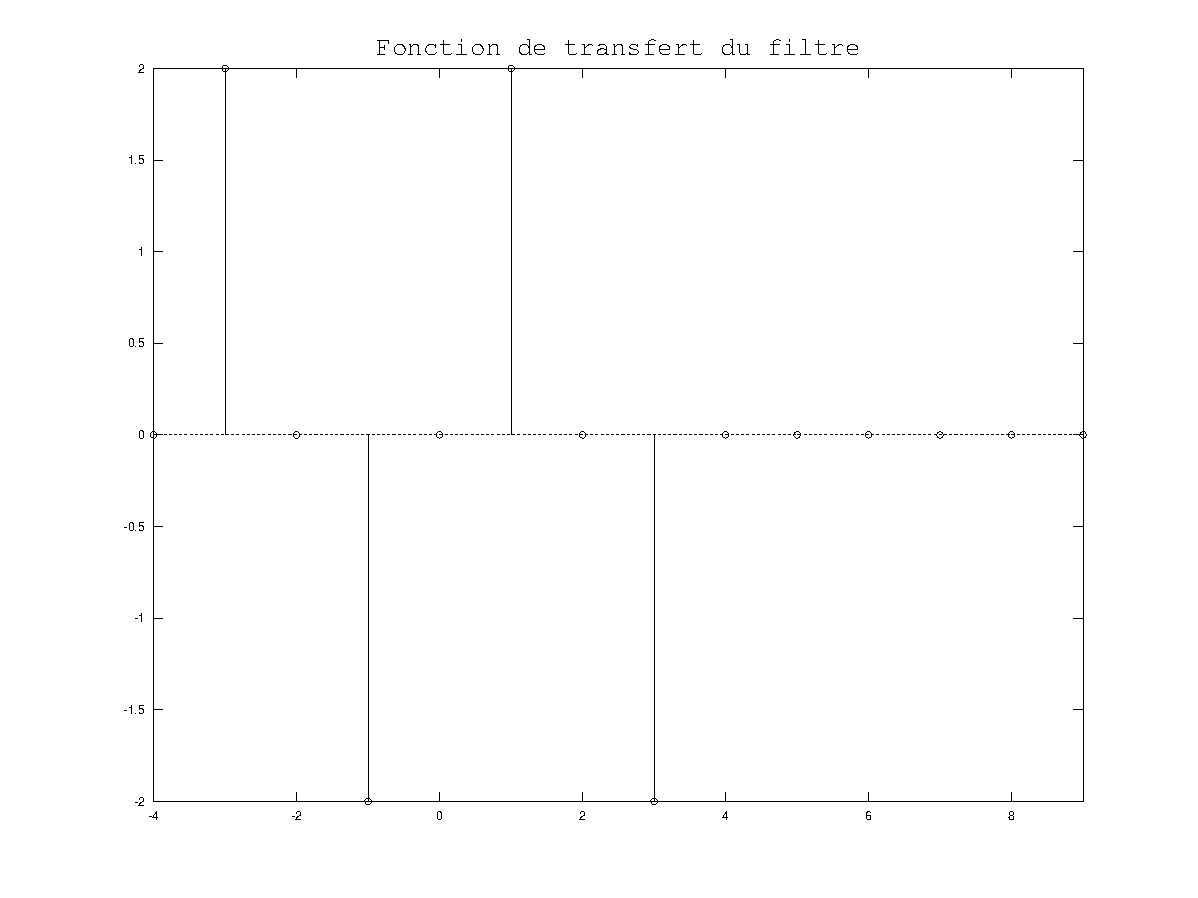
\includegraphics[width=9cm]{resEx2/fctTransfert.pdf}
\caption{Fonction de transfert du filtre $2*sin(\frac{n*\pi}{2})[u(n+3)-u(n-4)]$}
\end{figure}

Le signal d'entrée définit par la fonction $\frac{n}{2}[u(n)-u(n-6)]$ est le suivant:

\begin{figure}[H]
\centering
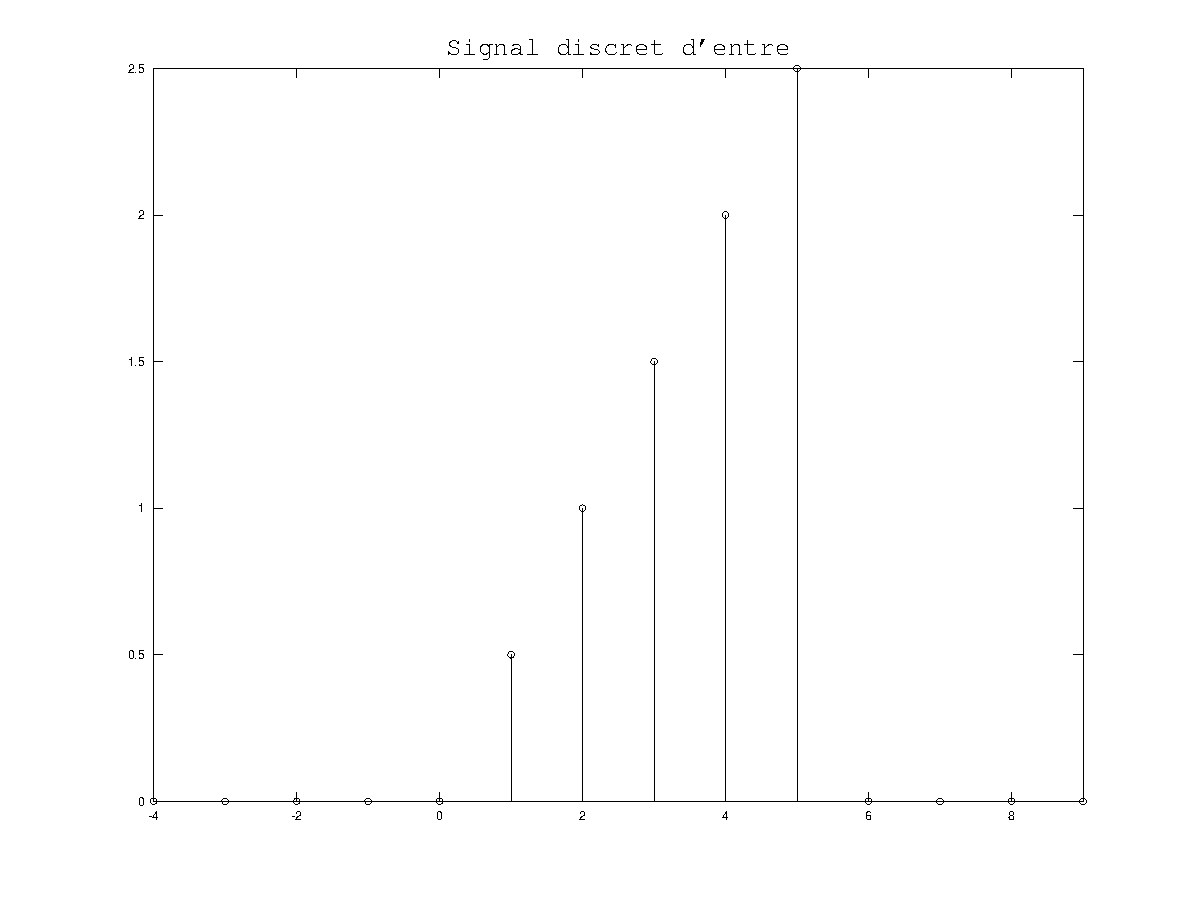
\includegraphics[width=9cm]{resEx2/signalEntree.pdf}
\caption{Signal d'entrée}
\end{figure}

La réponse impulsion du filtre précédent nous donne la figure suivante : 

\begin{figure}[H]
\centering
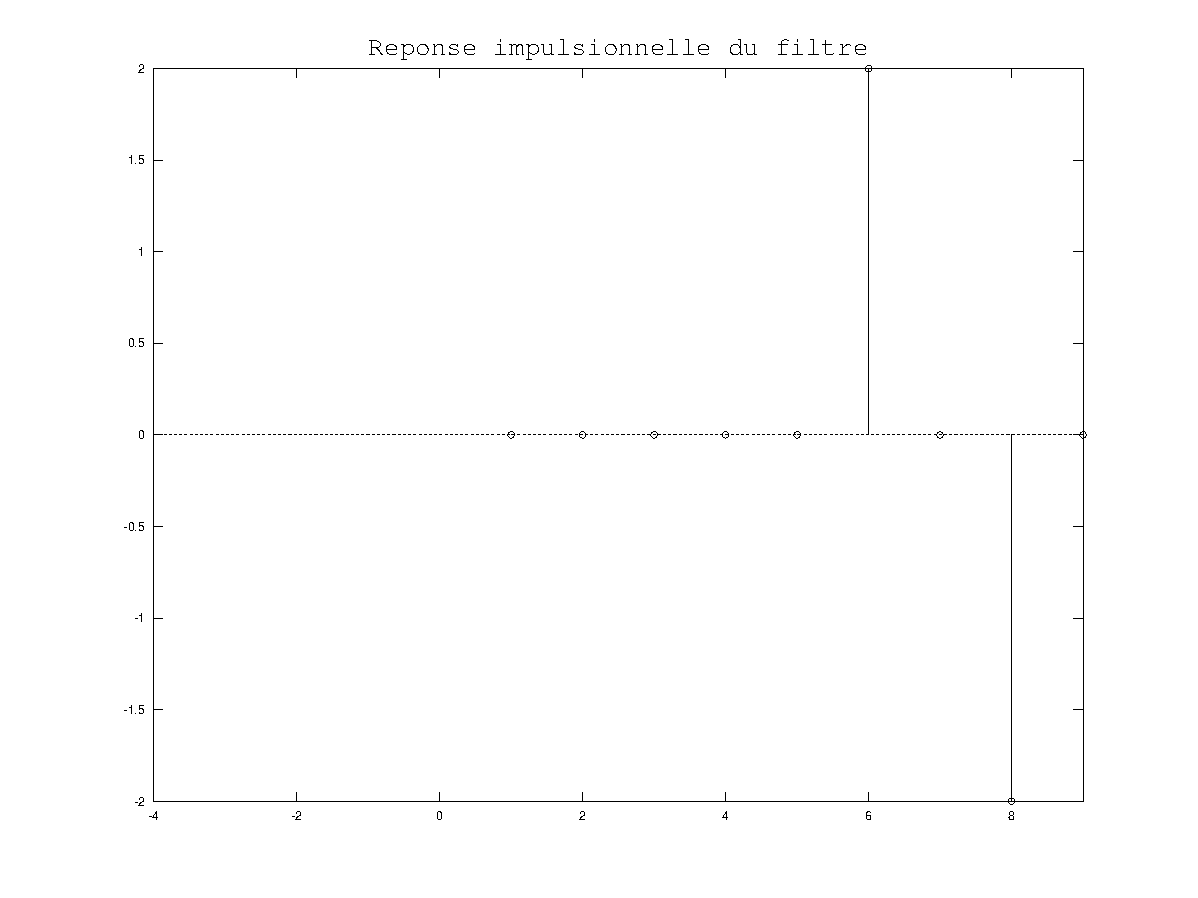
\includegraphics[width=9cm]{resEx2/repImpulsionnelle.pdf}
\caption{Réponse impulsionnelle du filtre}
\end{figure}

Le produit de convolution du filtre et du signal nous donne le signal ci dessous :

\begin{figure}[H]
\centering
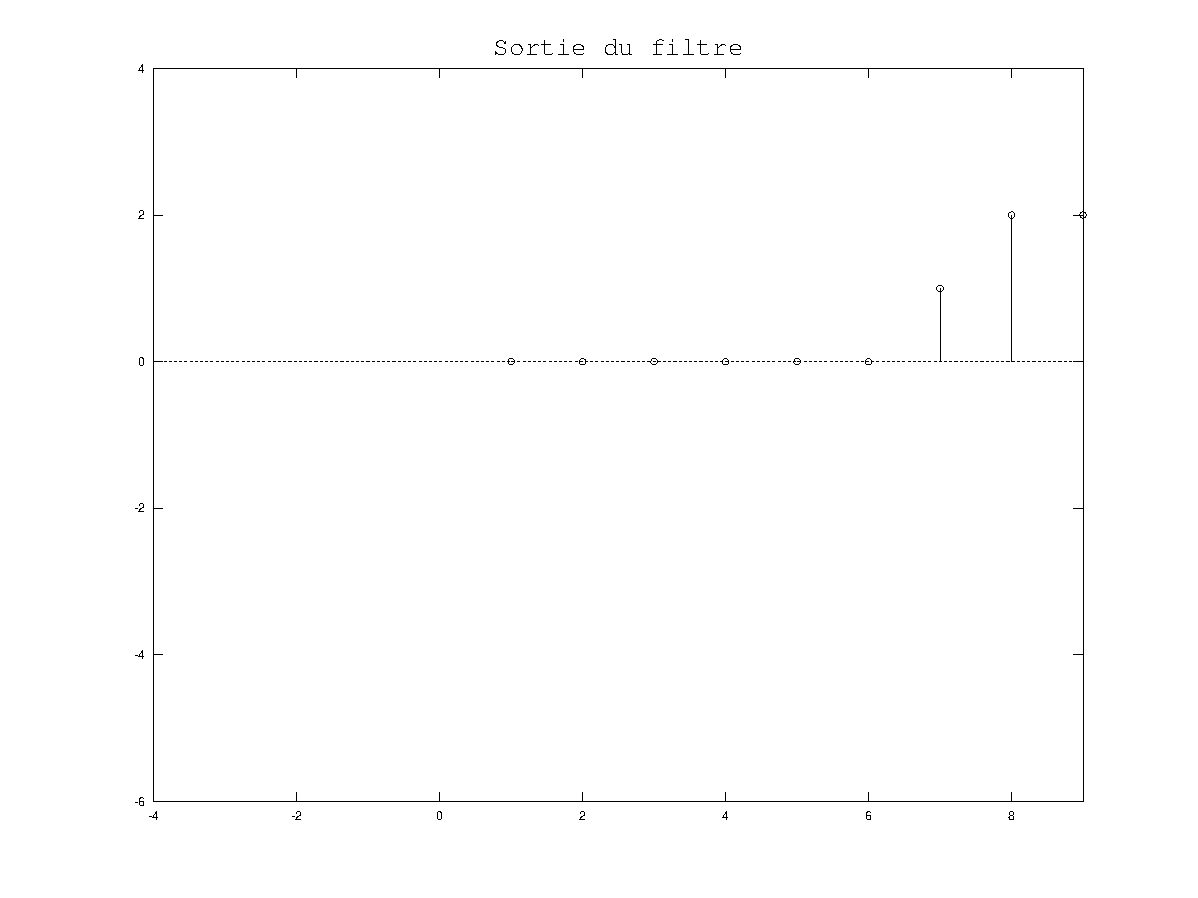
\includegraphics[width=9cm]{resEx2/sortieFiltre.pdf}
\caption{Signal en sortie du filtre}
\end{figure}

\part{Exercice 3}
\section{Fonction $\frac{1-z^{-1}}{2}$}
Nous commençons par afficher le diagramme de gain en décibel (\ref{f1 Diagramme de gain}) ainsi que le diagramme de phase en radians (\ref{f1 Diagramme de phase}) pour déterminer la nature du filtre représenté par cette fonction de transfert.
\begin{figure}[H]
\centering
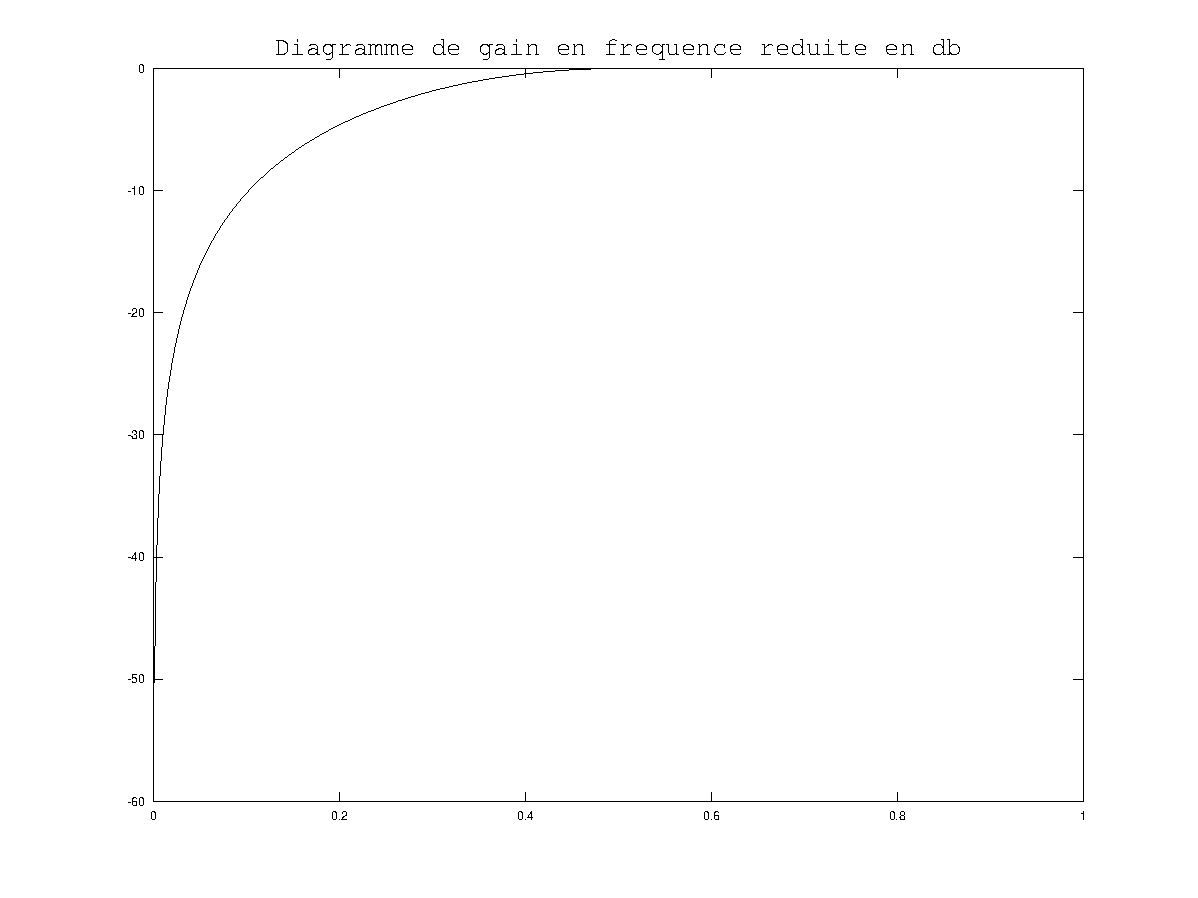
\includegraphics[width=9cm]{resEx3/f1Gain.pdf}
\caption{Diagramme de gain de la fonction $\frac{1-z^{-1}}{2}$ en dB}
\label{f1 Diagramme de gain}
\end{figure}
\begin{figure}[H]
\centering
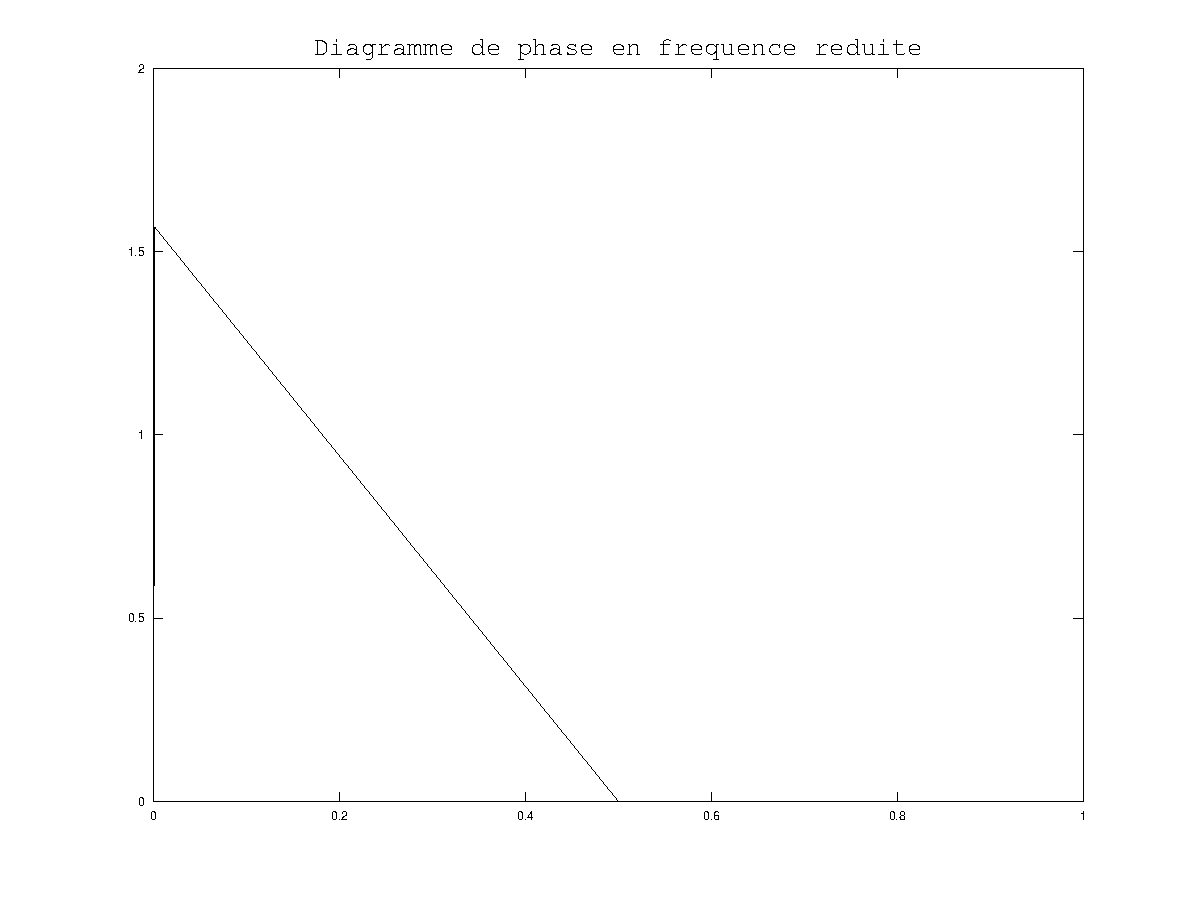
\includegraphics[width=9cm]{resEx3/f1Phase.pdf}
\caption{Diagramme de phase de la fonction $\frac{1-z^{-1}}{2}$ en radians}
\label{f1 Diagramme de phase}
\end{figure}
Nous pouvons donc constater que cette fonction de transfert en z correspond à un filtre passe haut.
\subsection{Réponse impulsionnelle}
~\\
\begin{figure}[H]
\centering
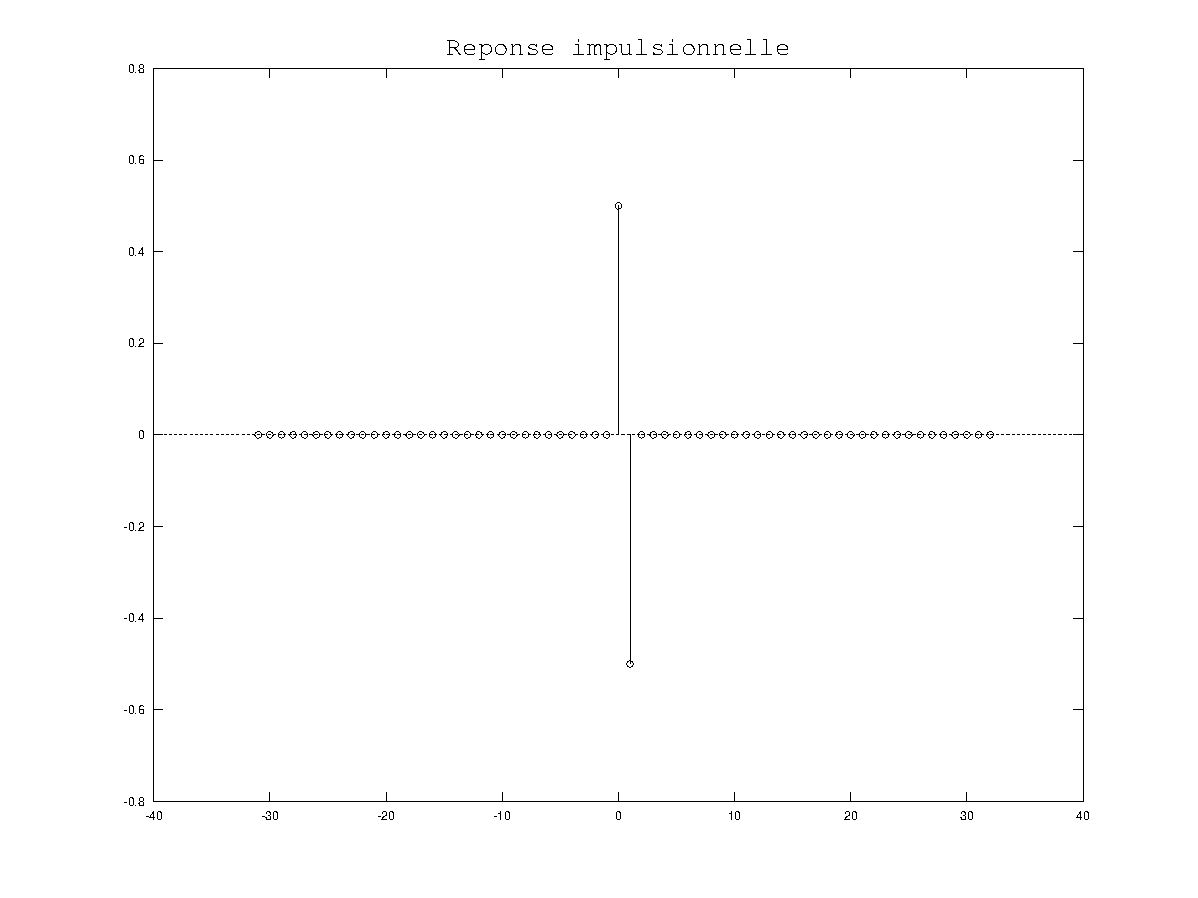
\includegraphics[width=9cm]{resEx3/f1Impulsion.pdf}
\caption{Réponse impulsionnelle de la fonction $\frac{1-z^{-1}}{2}$ }
\end{figure}
\subsection{Réponse indicielle}
~\\
\begin{figure}[H]
\centering
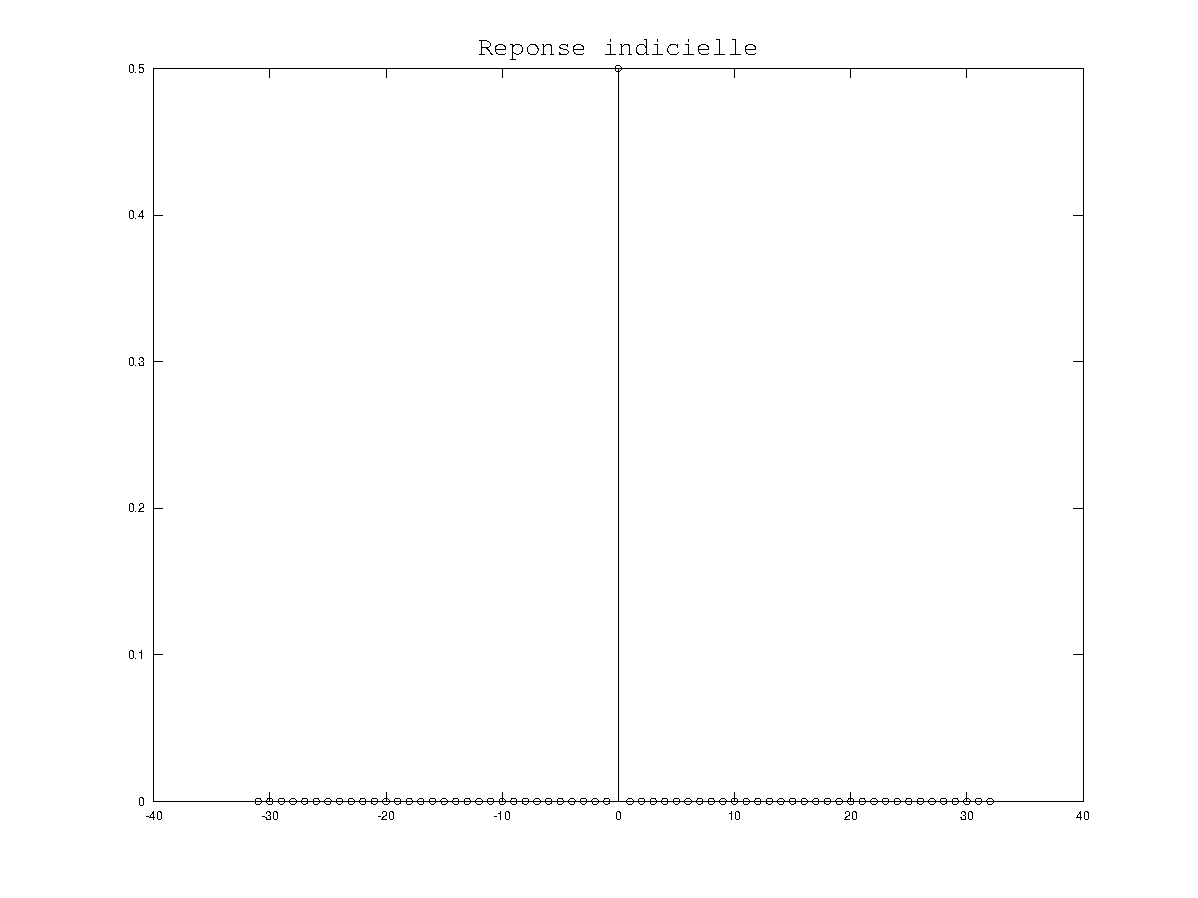
\includegraphics[width=9cm]{resEx3/f1Indice.pdf}
\caption{Réponse indicielle de la fonction $\frac{1-z^{-1}}{2}$ }
\end{figure}

\subsection{Les zéros et les pôles}
~\\
\begin{figure}[H]
\centering
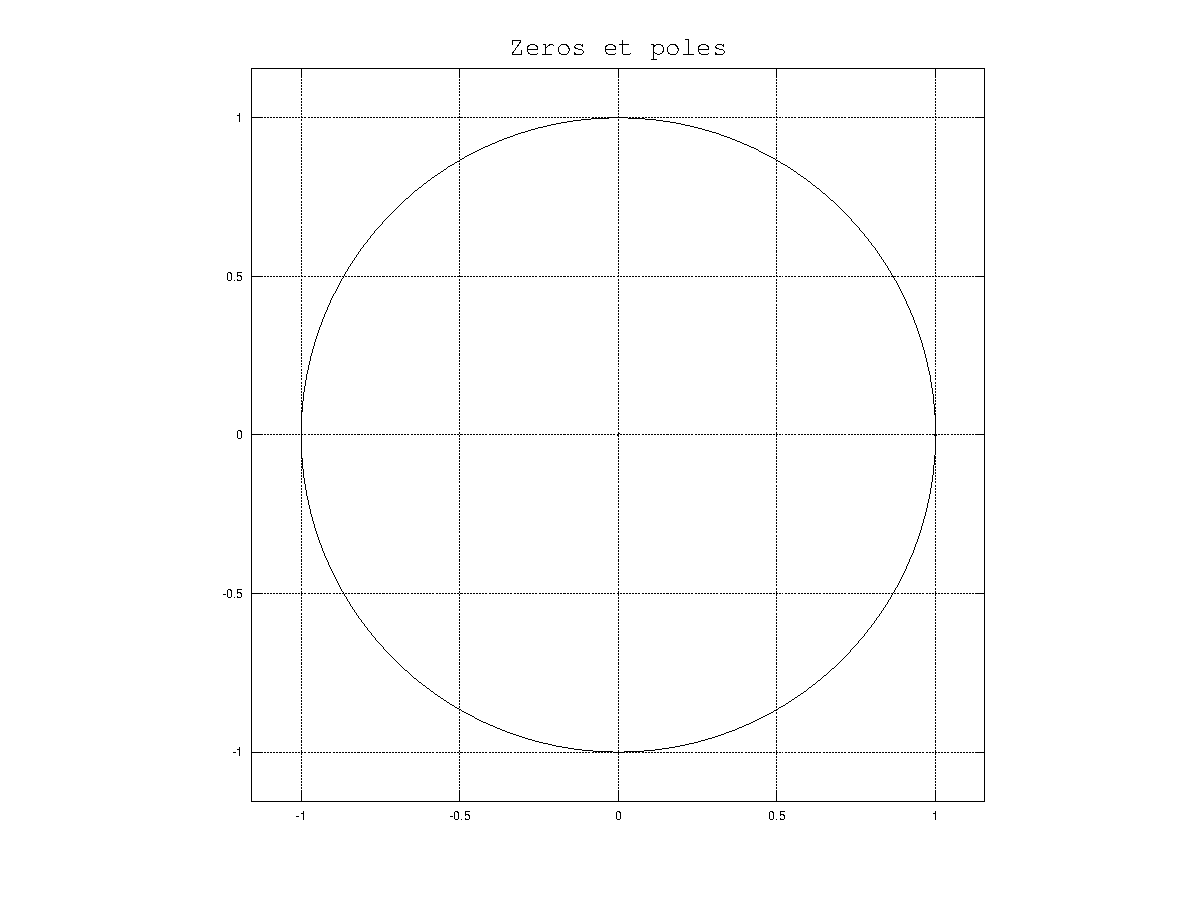
\includegraphics[width=9cm]{resEx3/f1ZP.pdf}
\caption{Les zéros et les pôles de la fonction $\frac{1-z^{-1}}{2}$ }
\end{figure}


\section{Fonction $\frac{1+z^{-1}}{2}$}
Nous commençons par afficher le diagramme de gain en décibel (\ref{f2 Diagramme de gain}) ainsi que le diagramme de phase en radians (\ref{f2 Diagramme de phase}) pour déterminer la nature du filtre représenté par cette fonction de transfert.
\begin{figure}[H]
\centering
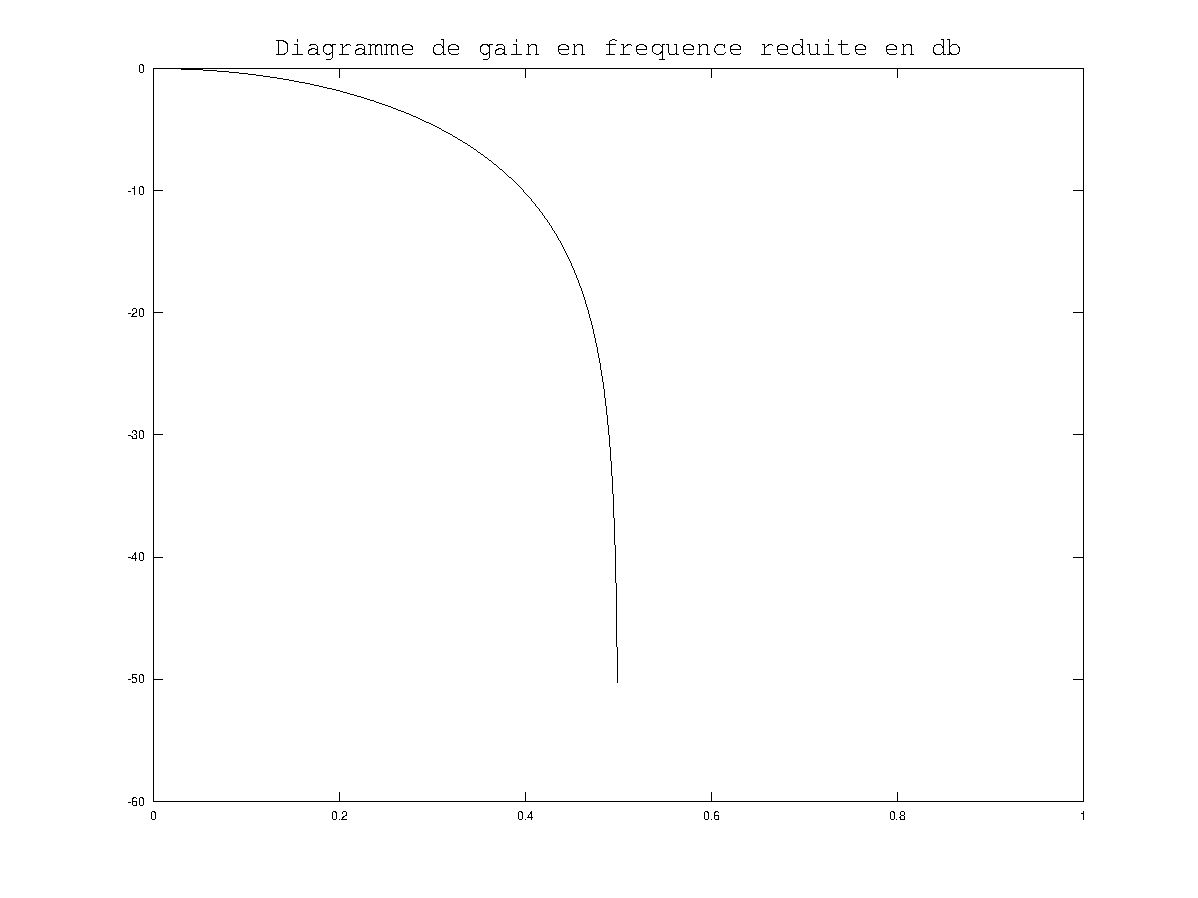
\includegraphics[width=9cm]{resEx3/f2Gain.pdf}
\caption{Diagramme de gain de la fonction $\frac{1+z^{-1}}{2}$ en dB}
\label{f2 Diagramme de gain}
\end{figure}
\begin{figure}[H]
\centering
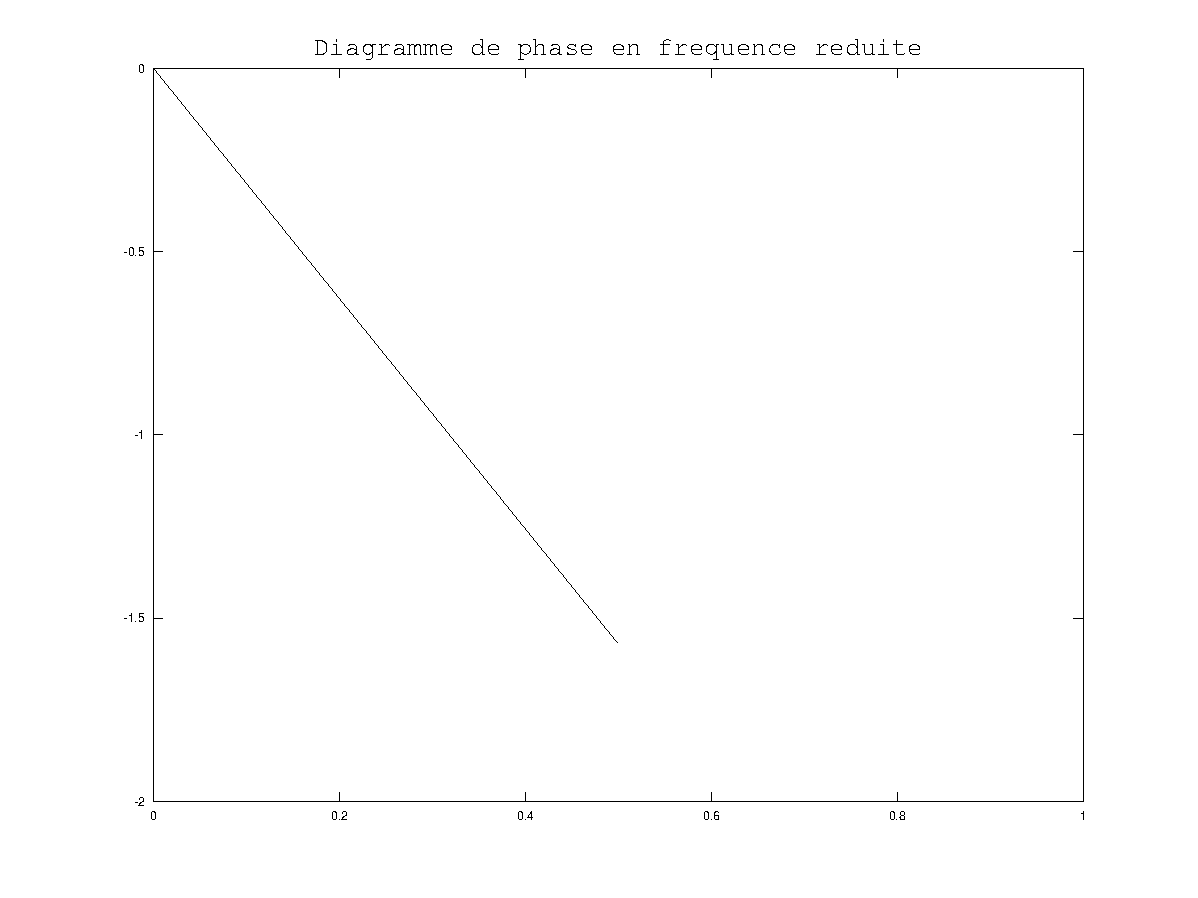
\includegraphics[width=9cm]{resEx3/f2Phase.pdf}
\caption{Diagramme de phase de la fonction $\frac{1+z^{-1}}{2}$ en radians}
\label{f2 Diagramme de phase}
\end{figure}
Nous pouvons donc constater que cette fonction de transfert en z correspond à un filtre passe bas.
\subsection{Réponse impulsionnelle}
~\\
\begin{figure}[H]
\centering
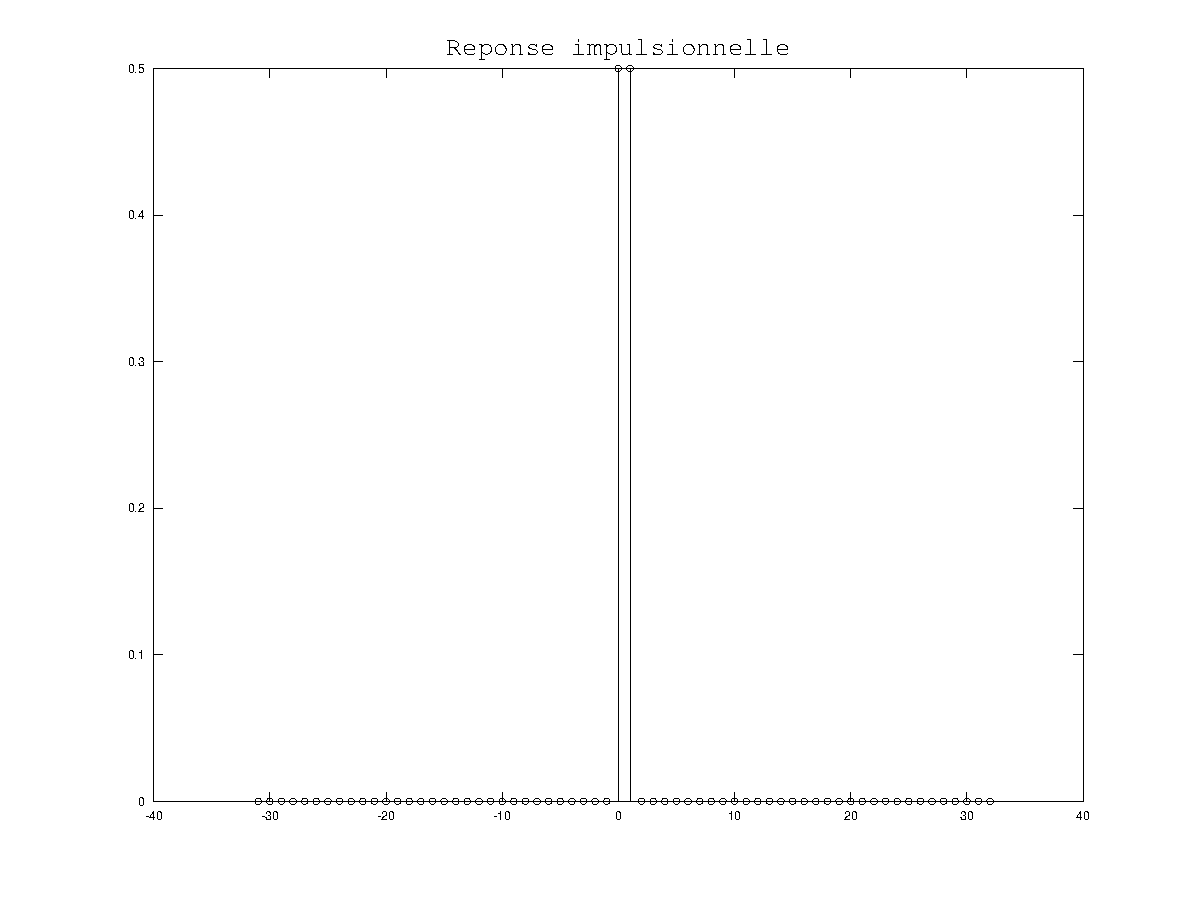
\includegraphics[width=9cm]{resEx3/f2Impulsion.pdf}
\caption{Réponse impulsionnelle de la fonction $\frac{1+z^{-1}}{2}$ }
\end{figure}

\subsection{Réponse indicielle}
~\\
\begin{figure}[H]
\centering
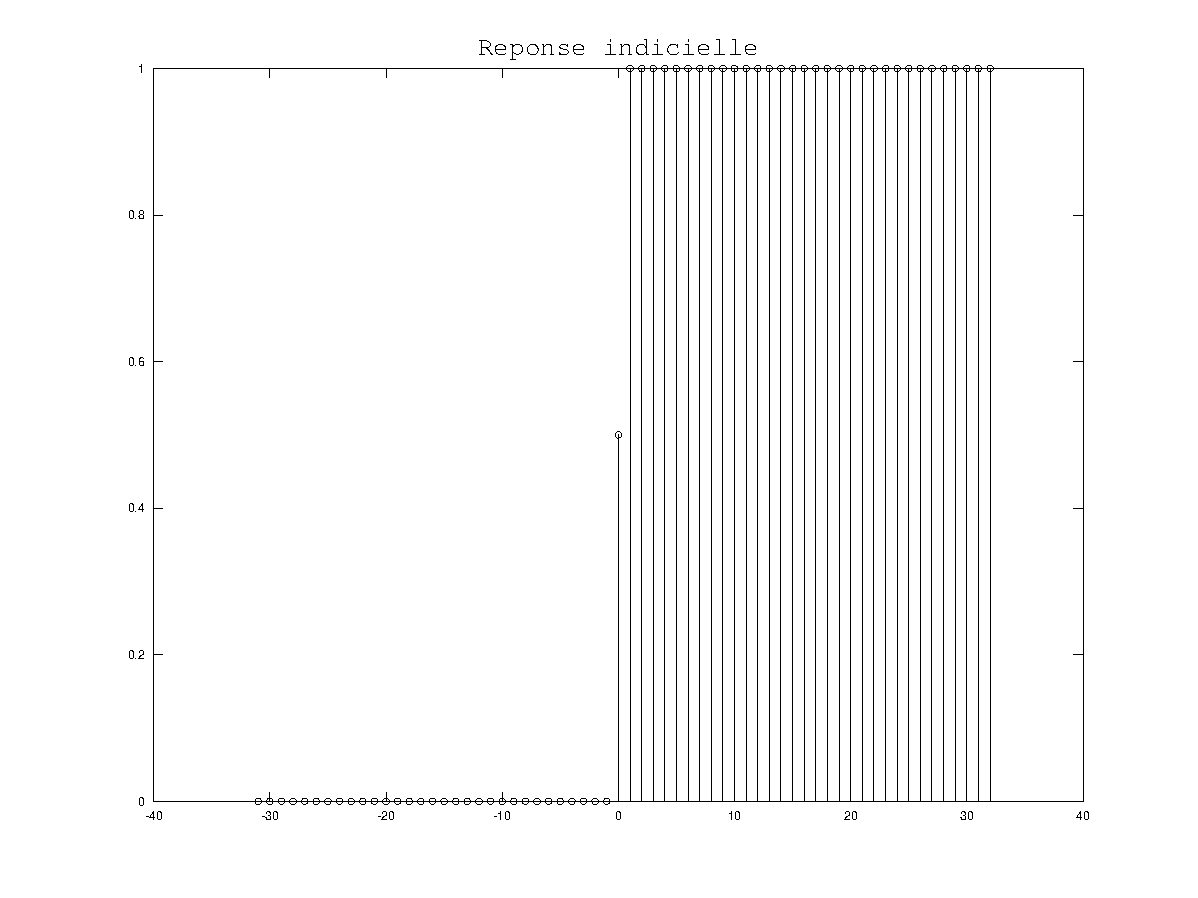
\includegraphics[width=9cm]{resEx3/f2Indice.pdf}
\caption{Réponse indicielle de la fonction $\frac{1+z^{-1}}{2}$ }
\end{figure}

\subsection{Les zéros et les pôles}
~\\
\begin{figure}[H]
\centering
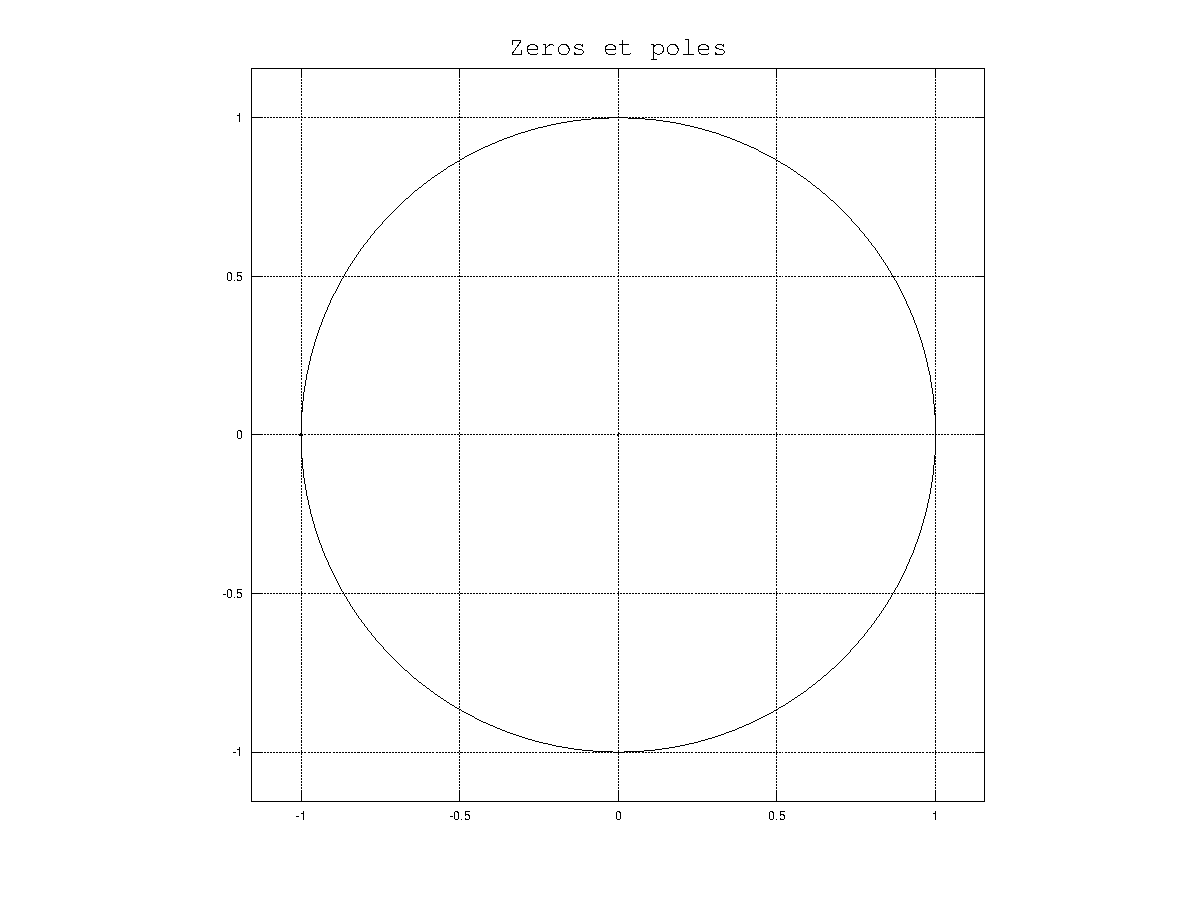
\includegraphics[width=9cm]{resEx3/f2ZP.pdf}
\caption{Les zéros et les pôles de la fonction $\frac{1+z^{-1}}{2}$ }
\end{figure}


\section{Fonction $\frac{1-z^{-2}}{2}$}
Nous commençons par afficher le diagramme de gain en décibel (\ref{f3 Diagramme de gain}) ainsi que le diagramme de phase en radians (\ref{f3 Diagramme de phase}) pour déterminer la nature du filtre représenté par cette fonction de transfert.
\begin{figure}[H]
\centering
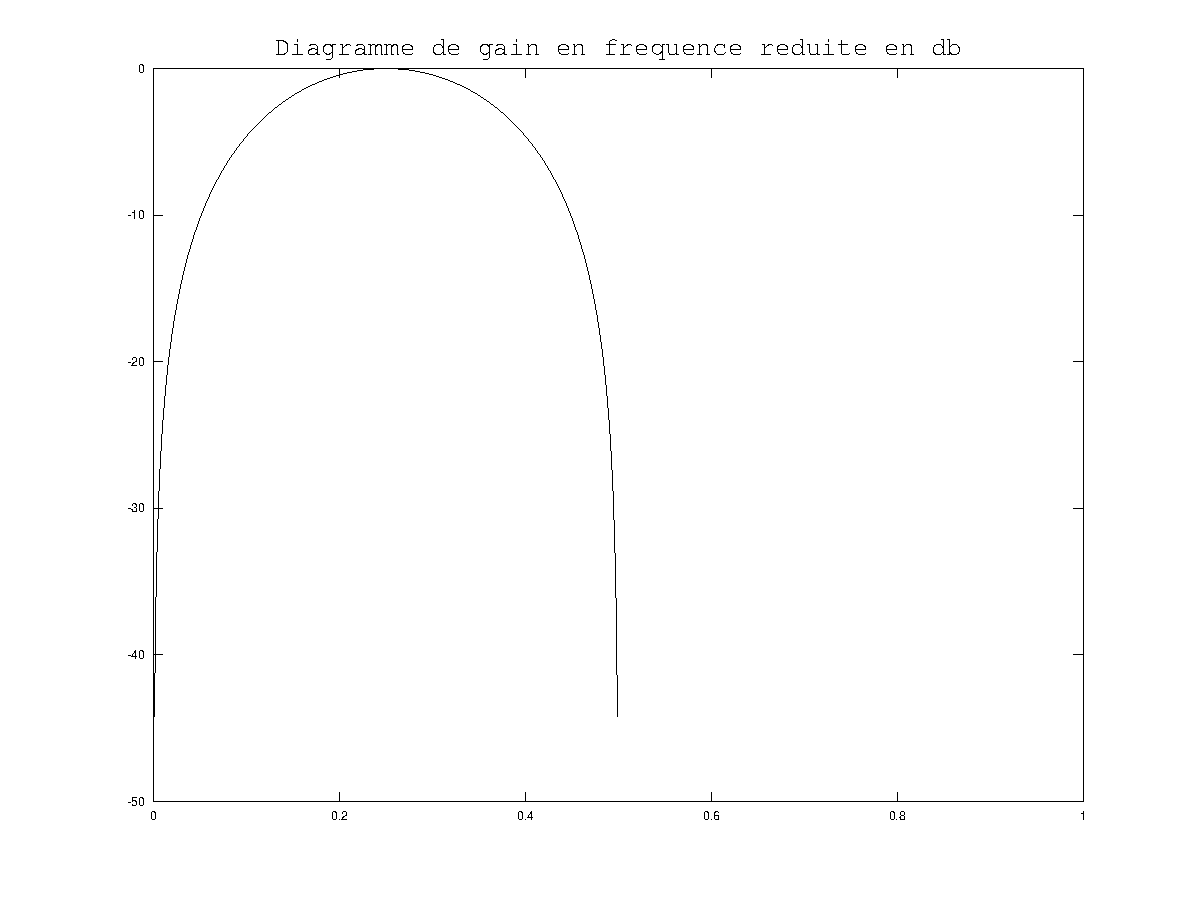
\includegraphics[width=9cm]{resEx3/f3Gain.pdf}
\caption{Diagramme de gain de la fonction $\frac{1-z^{-2}}{2}$ en dB}
\label{f3 Diagramme de gain}
\end{figure}
\begin{figure}[H]
\centering
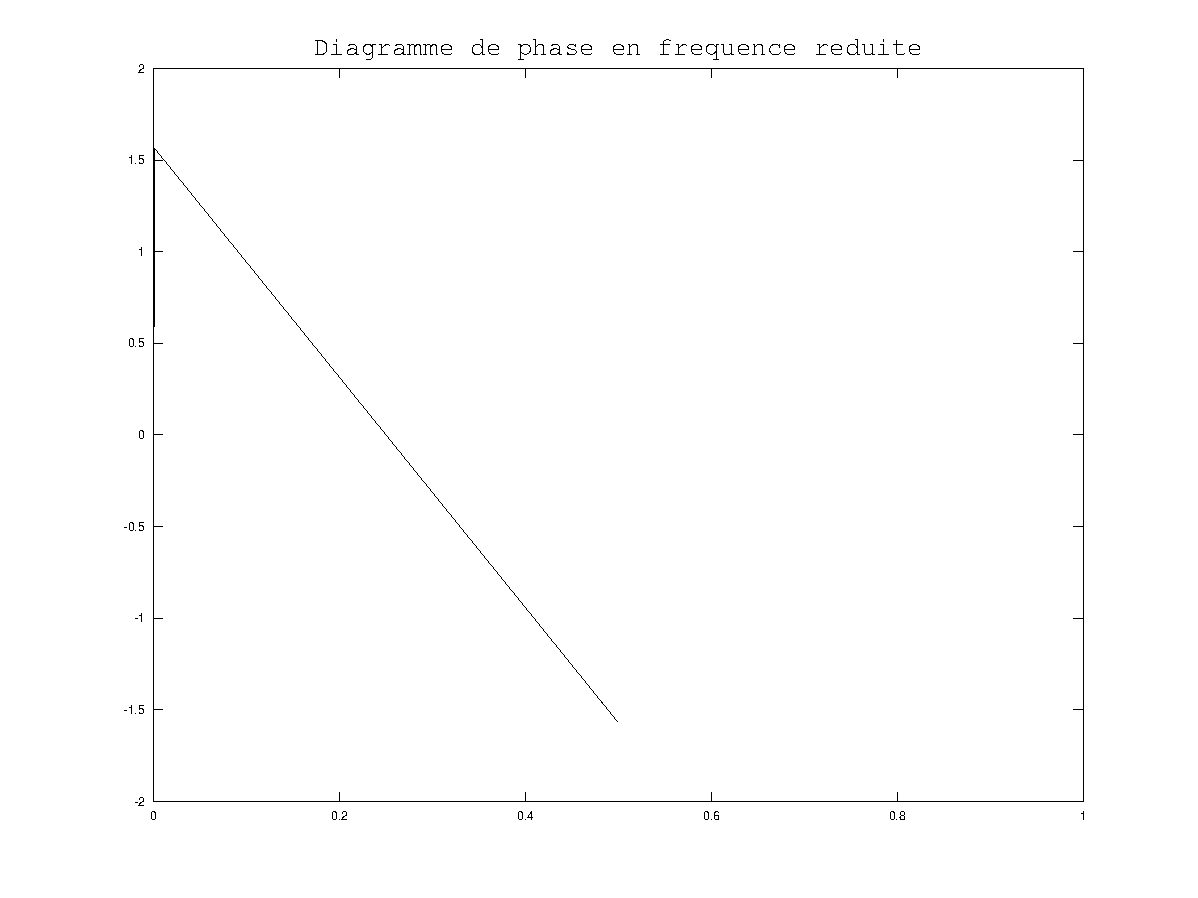
\includegraphics[width=9cm]{resEx3/f3Phase.pdf}
\caption{Diagramme de phase de la fonction $\frac{1-z^{-2}}{2}$ en radians}
\label{f3 Diagramme de phase}
\end{figure}
Nous pouvons donc constater que cette fonction de transfert en z correspond à un filtre passe bande.
\subsection{Réponse impulsionnelle}
~\\
\begin{figure}[H]
\centering
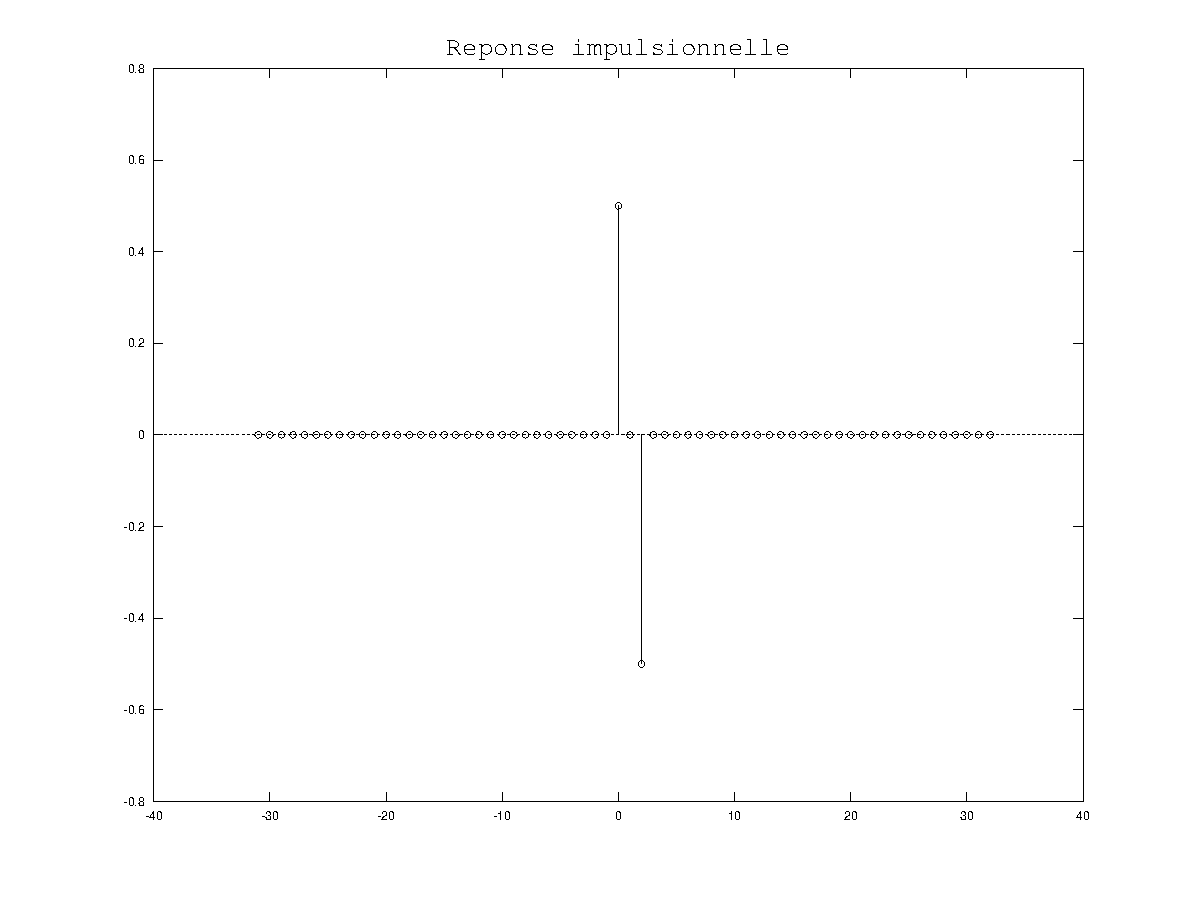
\includegraphics[width=9cm]{resEx3/f3Impulsion.pdf}
\caption{Réponse impulsionnelle de la fonction $\frac{1-z^{-2}}{2}$ }
\end{figure}

\subsection{Réponse indicielle}
~\\
\begin{figure}[H]
\centering
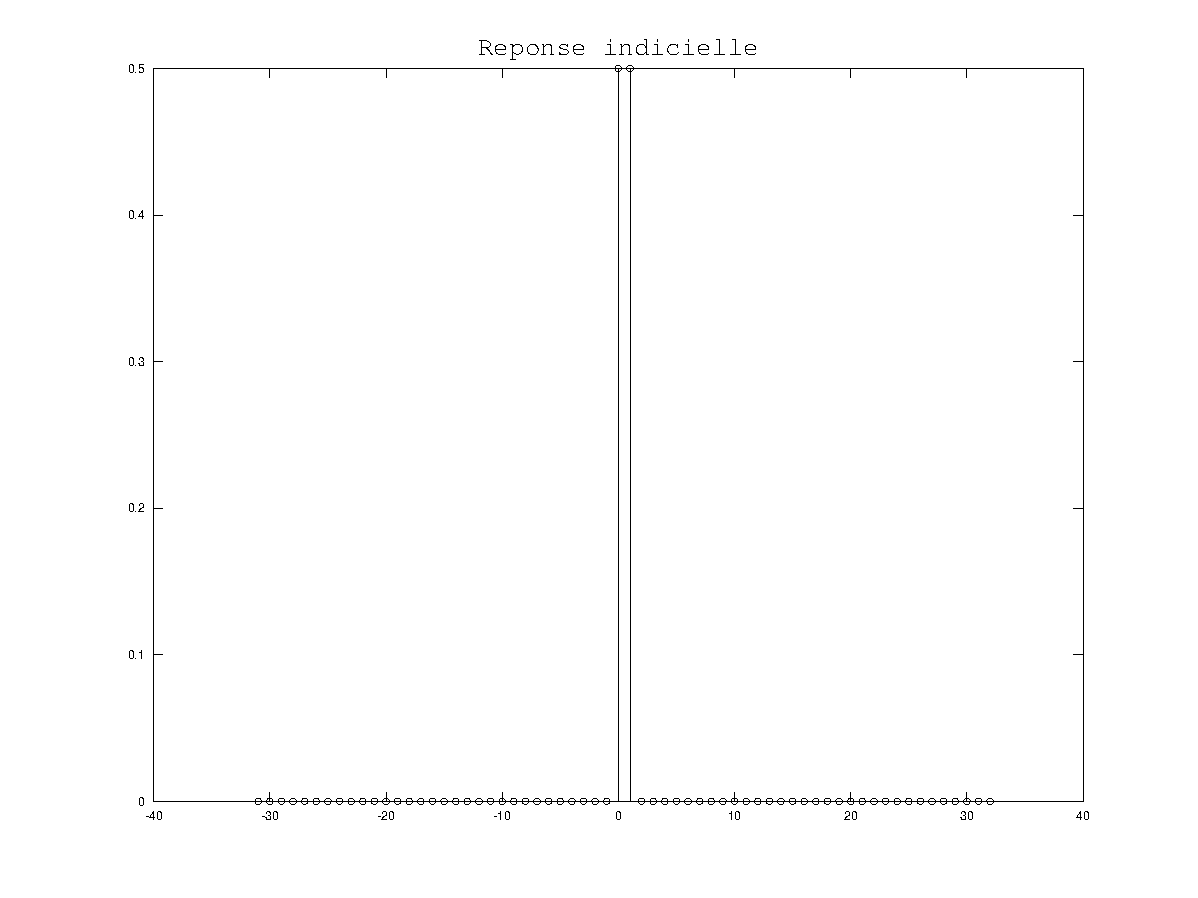
\includegraphics[width=9cm]{resEx3/f3Indice.pdf}
\caption{Réponse indicielle de la fonction $\frac{1-z^{-2}}{2}$ }
\end{figure}

\subsection{Les zéros et les pôles}
~\\
\begin{figure}[H]
\centering
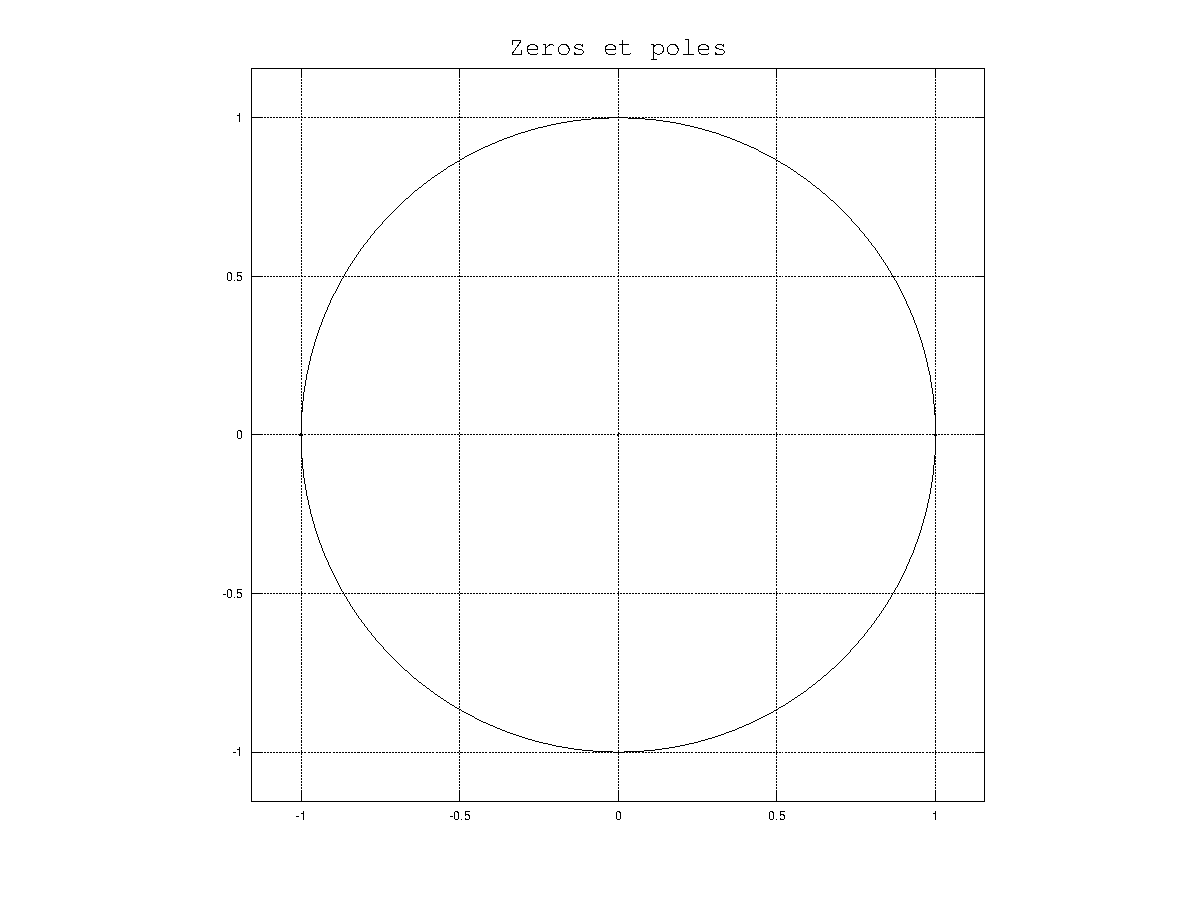
\includegraphics[width=9cm]{resEx3/f3ZP.pdf}
\caption{Les zéros et les pôles de la fonction $\frac{1-z^{-2}}{2}$ }
\end{figure}


\section{Fonction $\frac{2z^{-1}}{2-z^{-1}}$}
Nous commençons par afficher le diagramme de gain en décibel (\ref{f4 Diagramme de gain}) ainsi que le diagramme de phase en radians (\ref{f4 Diagramme de phase}) pour déterminer la nature du filtre représenté par cette fonction de transfert.
\begin{figure}[H]
\centering
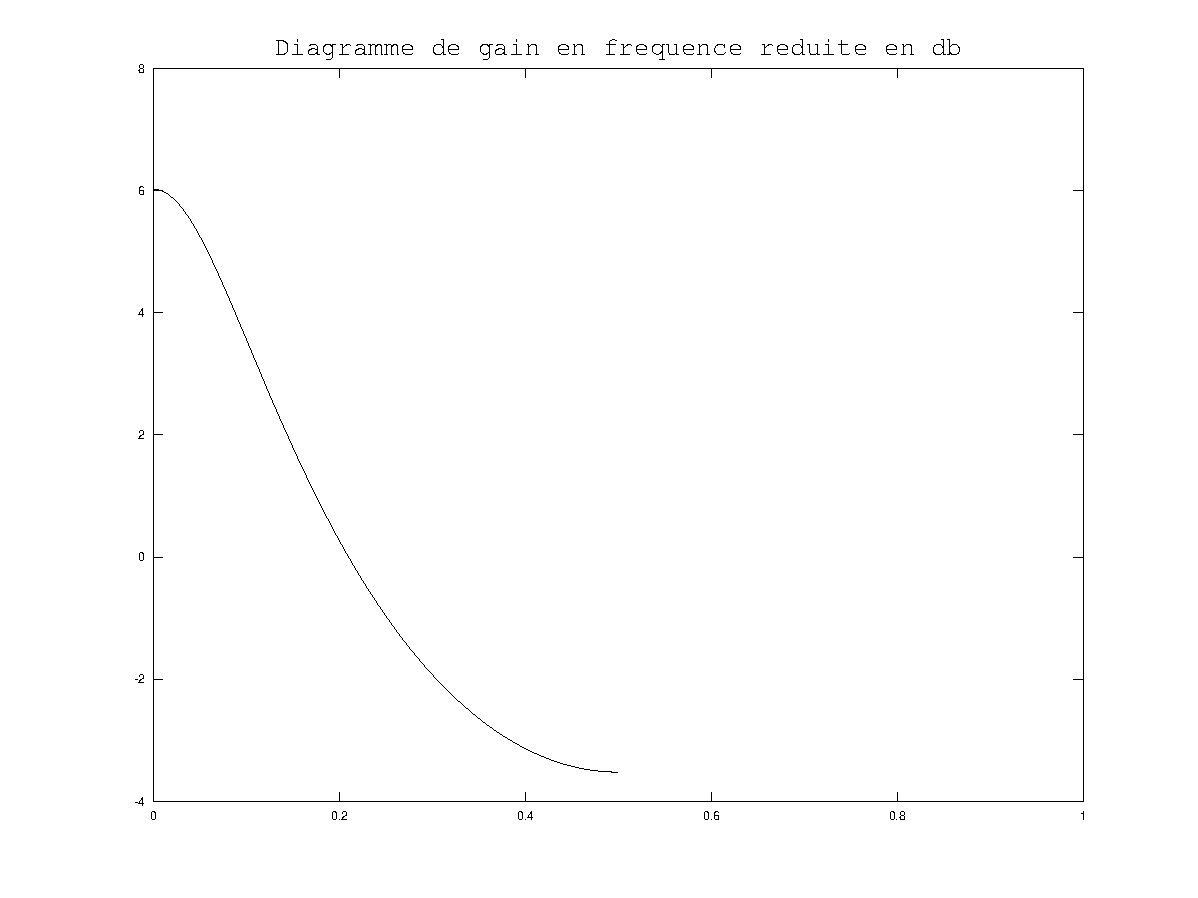
\includegraphics[width=9cm]{resEx3/f4Gain.pdf}
\caption{Diagramme de gain de la fonction $\frac{2z^{-1}}{2-z^{-1}}$ en dB}
\label{f4 Diagramme de gain}
\end{figure}
\begin{figure}[H]
\centering
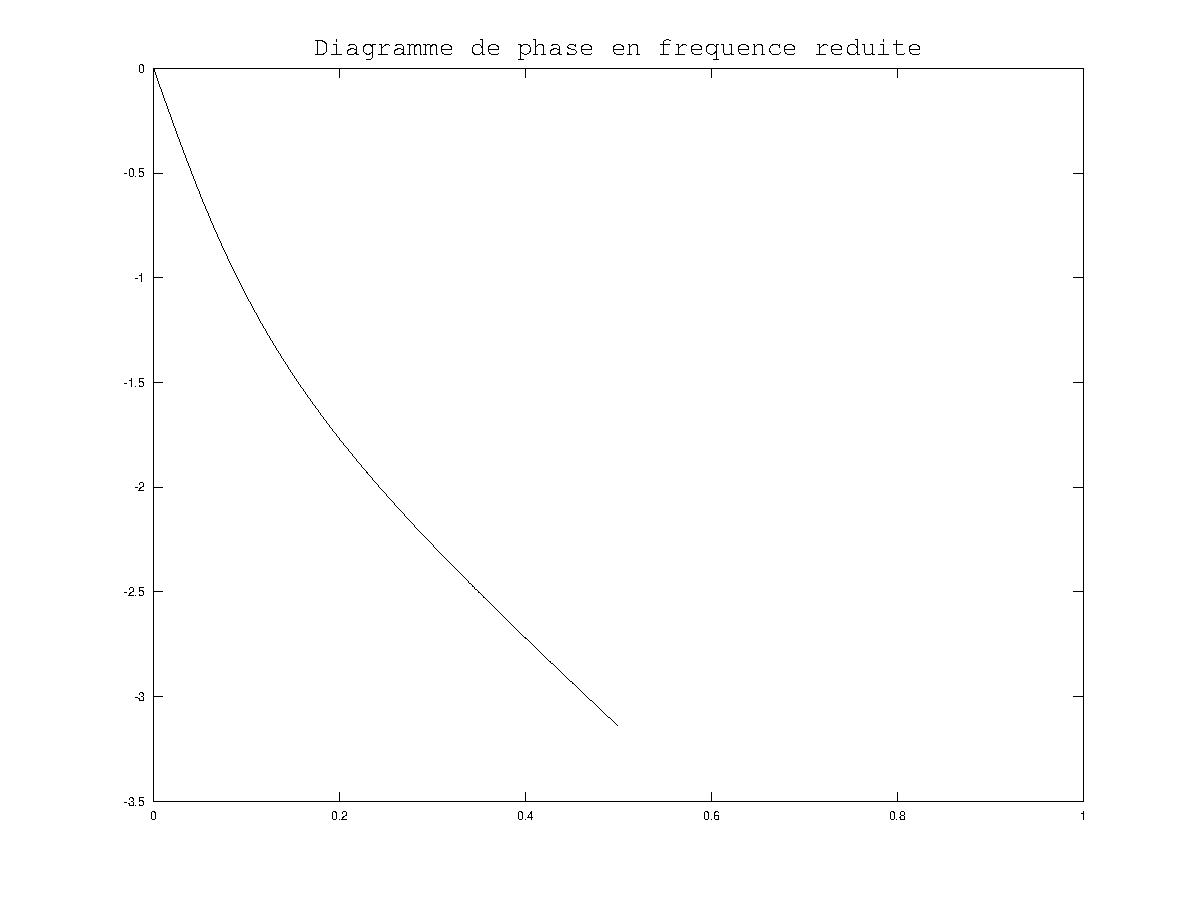
\includegraphics[width=9cm]{resEx3/f4Phase.pdf}
\caption{Diagramme de phase de la fonction $\frac{2z^{-1}}{2-z^{-1}}$ en radians}
\label{f4 Diagramme de phase}
\end{figure}
Nous pouvons donc constater que cette fonction de transfert en z correspond à un filtre passe bas.
\subsection{Réponse impulsionnelle}
~\\
\begin{figure}[H]
\centering
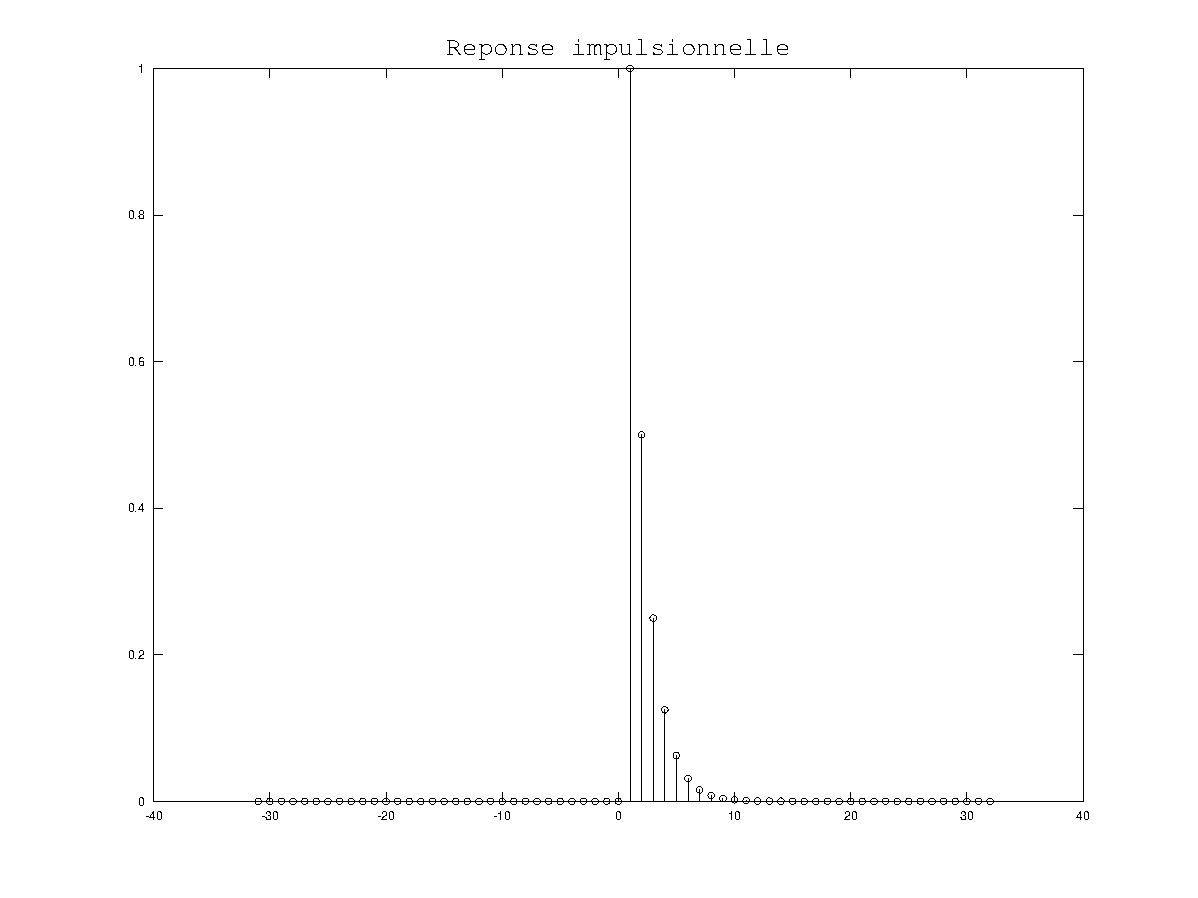
\includegraphics[width=9cm]{resEx3/f4Impulsion.pdf}
\caption{Réponse impulsionnelle de la fonction $\frac{2z^{-1}}{2-z^{-1}}$}
\end{figure}

\subsection{Réponse indicielle}
~\\
\begin{figure}[H]
\centering
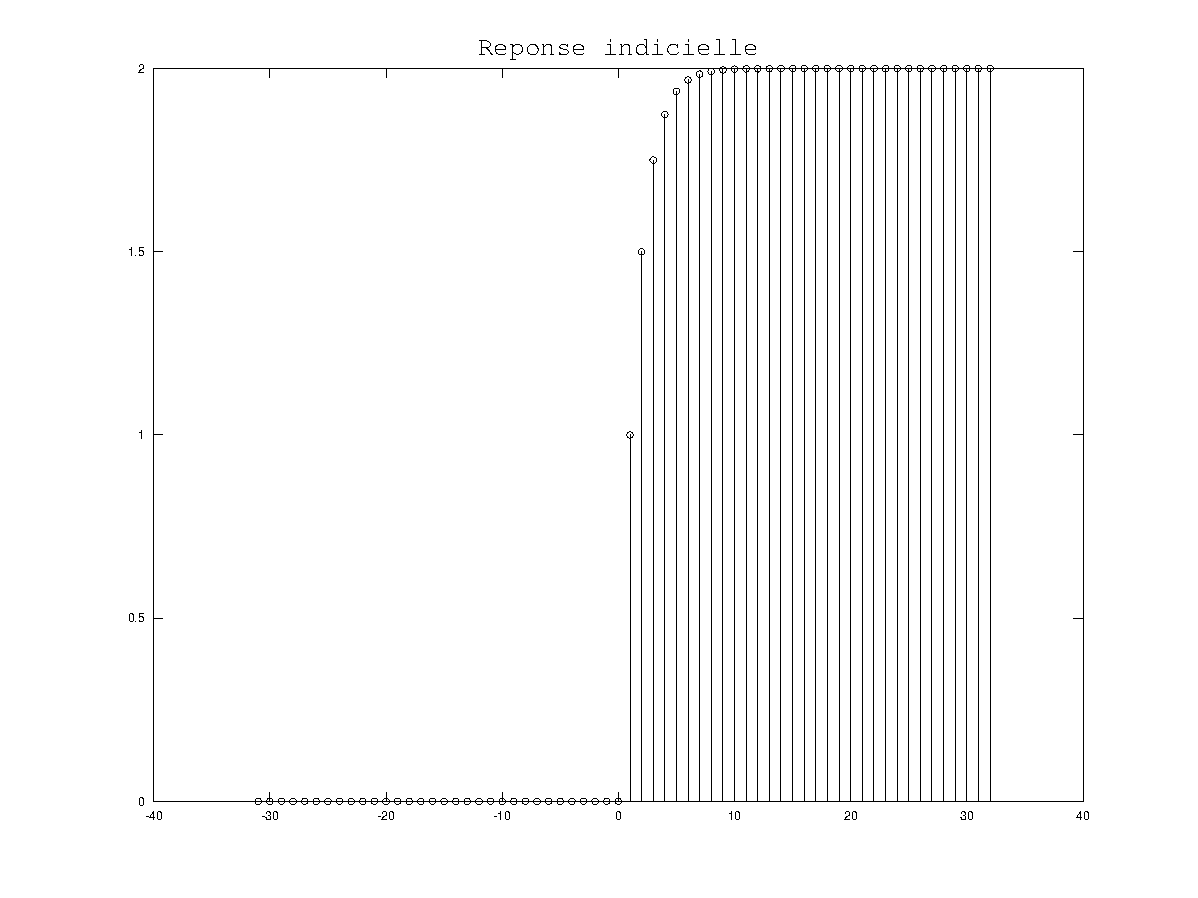
\includegraphics[width=9cm]{resEx3/f4Indice.pdf}
\caption{Réponse indicielle de la fonction $\frac{2z^{-1}}{2-z^{-1}}$}
\end{figure}

\subsection{Les zéros et les pôles}
~\\
\begin{figure}[H]
\centering
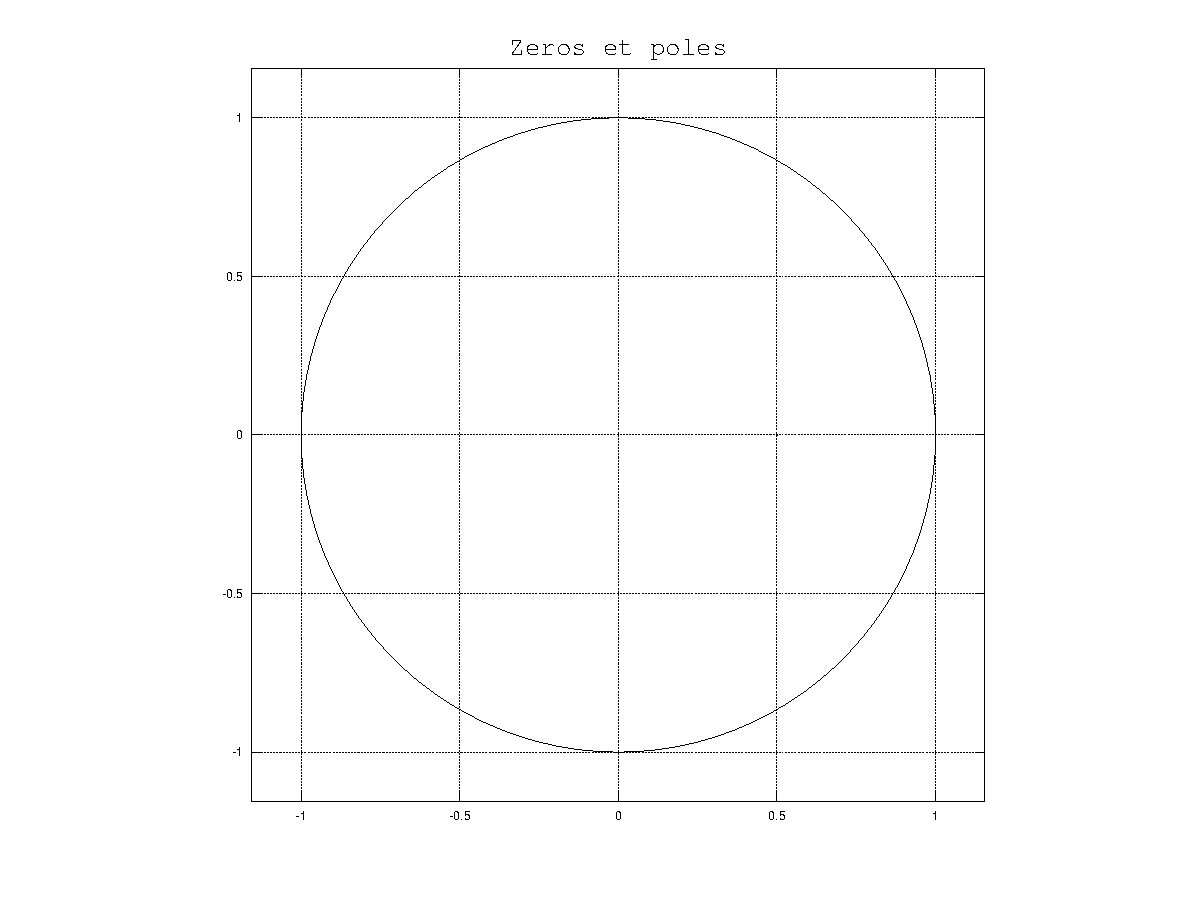
\includegraphics[width=9cm]{resEx3/f4ZP.pdf}
\caption{Les zéros et les pôles de la fonction $\frac{2z^{-1}}{2-z^{-1}}$ }
\end{figure}


\section{Fonction $\frac{2z^{-1}-z^{-5}}{2-z^{-1}}$}
Nous commençons par afficher le diagramme de gain en décibel (\ref{f5 Diagramme de gain}) ainsi que le diagramme de phase en radians (\ref{f5 Diagramme de phase}) pour déterminer la nature du filtre représenté par cette fonction de transfert.
\begin{figure}[H]
\centering
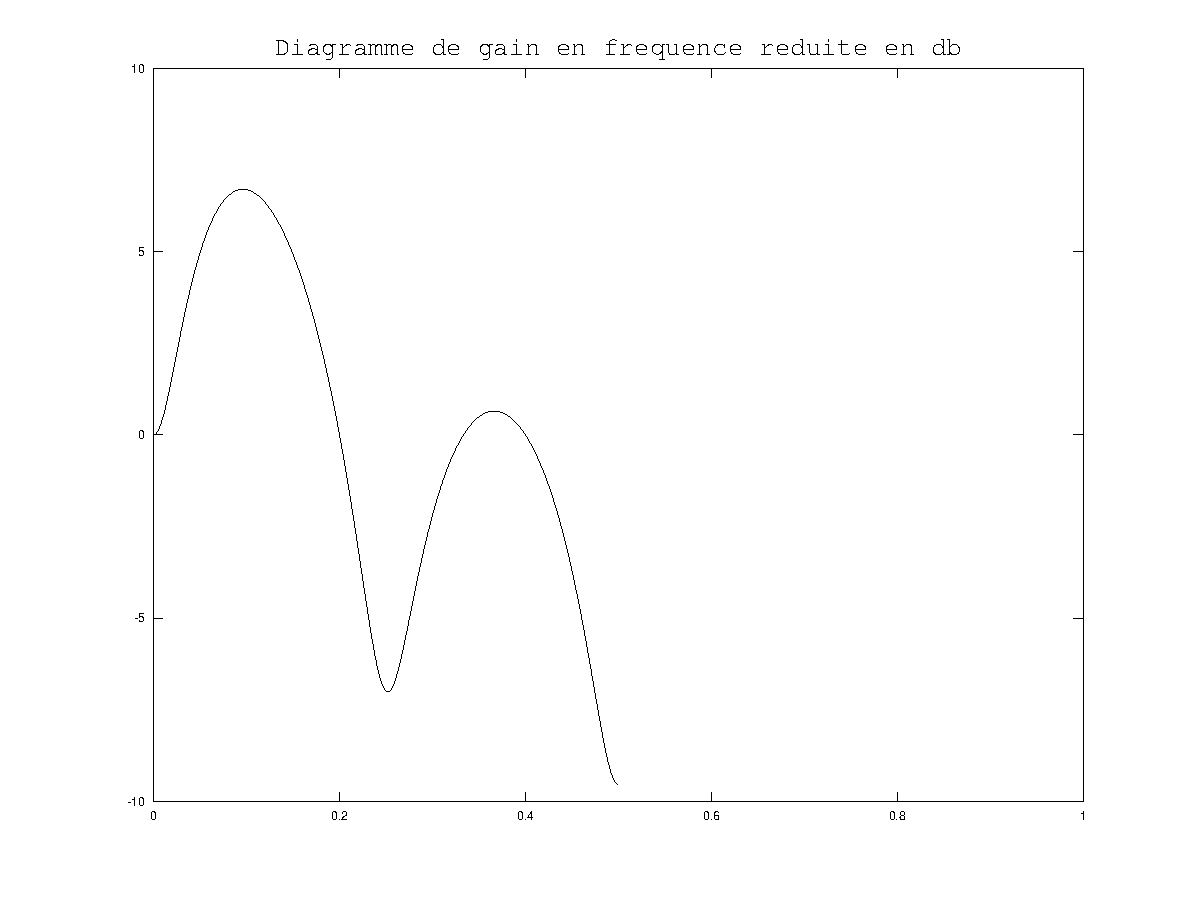
\includegraphics[width=9cm]{resEx3/f5Gain.pdf}
\caption{Diagramme de gain de la fonction $\frac{2z^{-1}-z^{-5}}{2-z^{-1}}$ en dB}
\label{f5 Diagramme de gain}
\end{figure}
\begin{figure}[H]
\centering
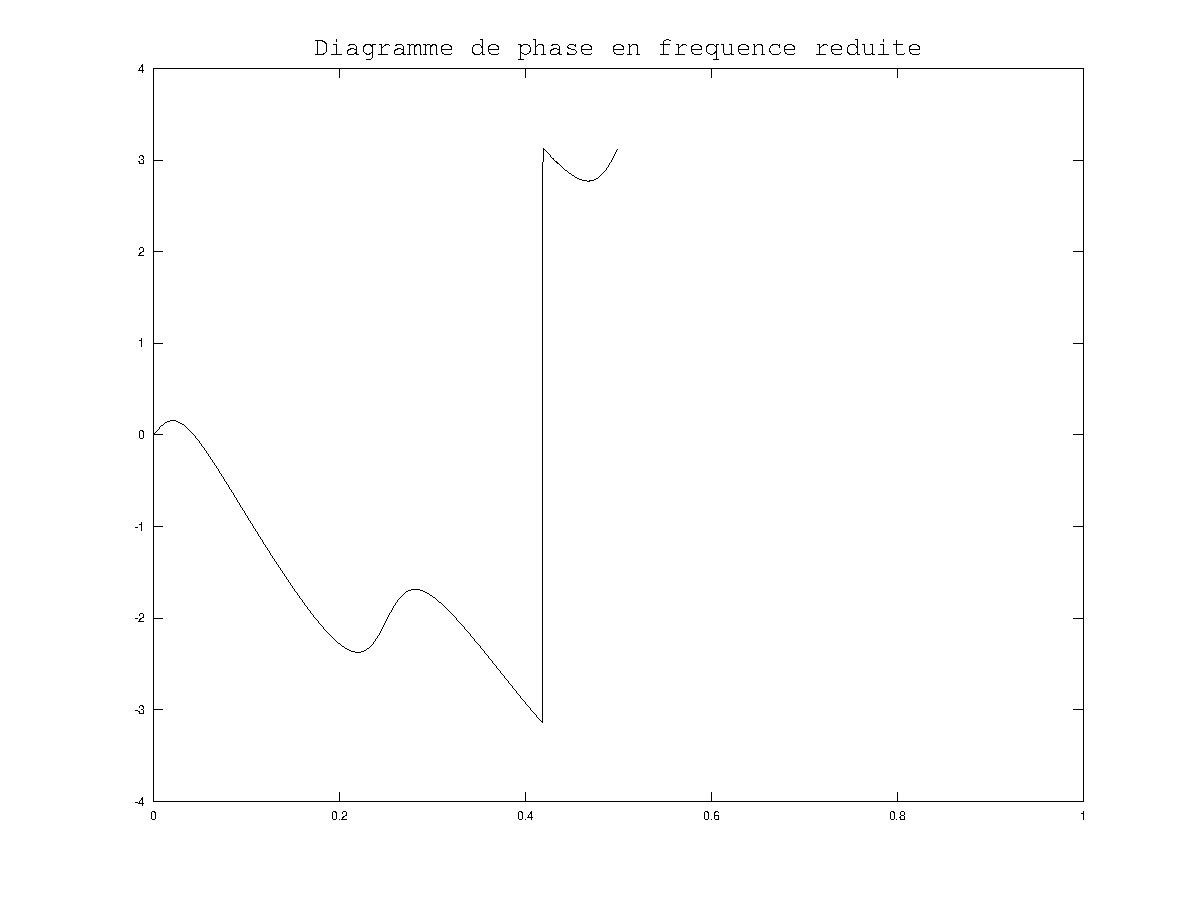
\includegraphics[width=9cm]{resEx3/f5Phase.pdf}
\caption{Diagramme de phase de la fonction $\frac{2z^{-1}-z^{-5}}{2-z^{-1}}$ en radians}
\label{f5 Diagramme de phase}
\end{figure}
Nous pouvons donc constater que cette fonction de transfert en z correspond à un filtre coupe bande.
\subsection{Réponse impulsionnelle}
~\\
\begin{figure}[H]
\centering
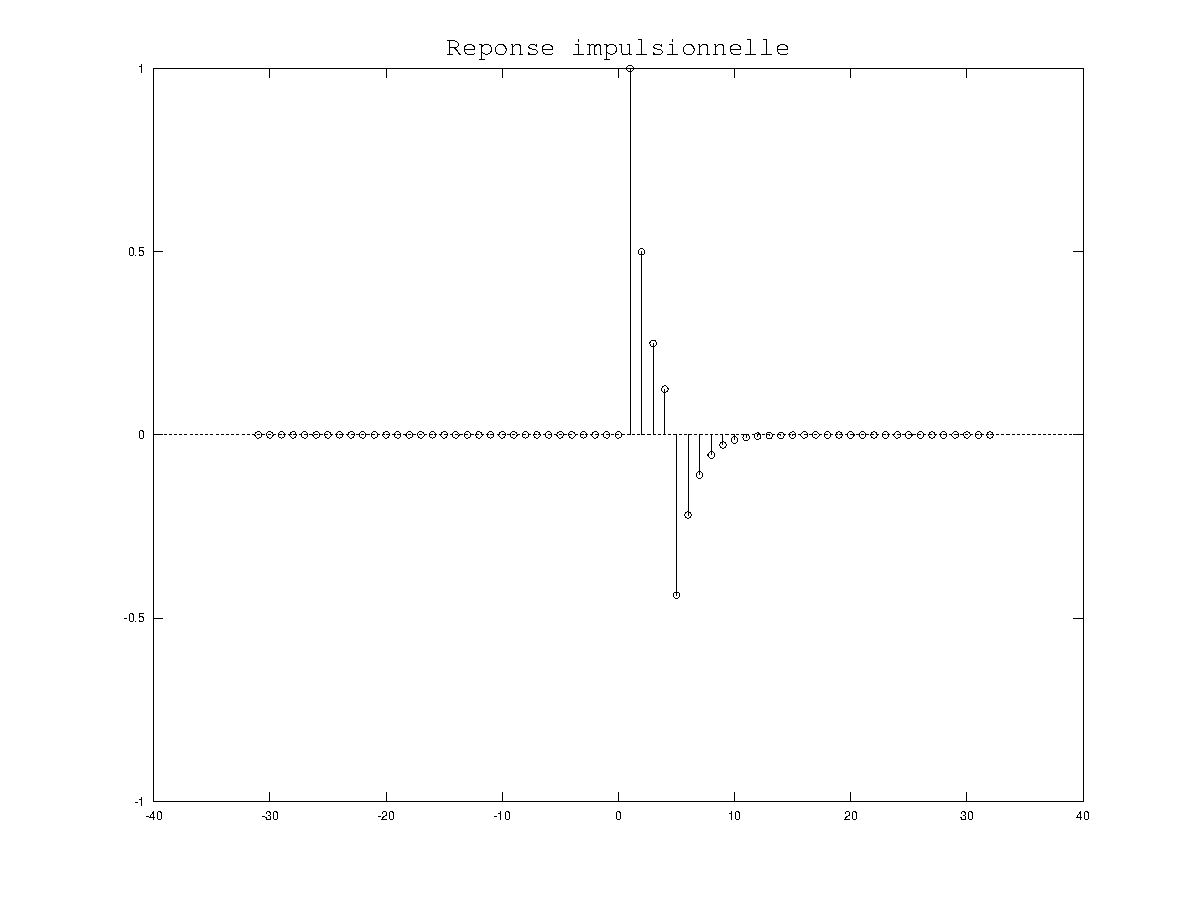
\includegraphics[width=9cm]{resEx3/f5Impulsion.pdf}
\caption{Réponse impulsionnelle de la fonction $\frac{2z^{-1}-z^{-5}}{2-z^{-1}}$ }
\end{figure}

\subsection{Réponse indicielle}
~\\
\begin{figure}[H]
\centering
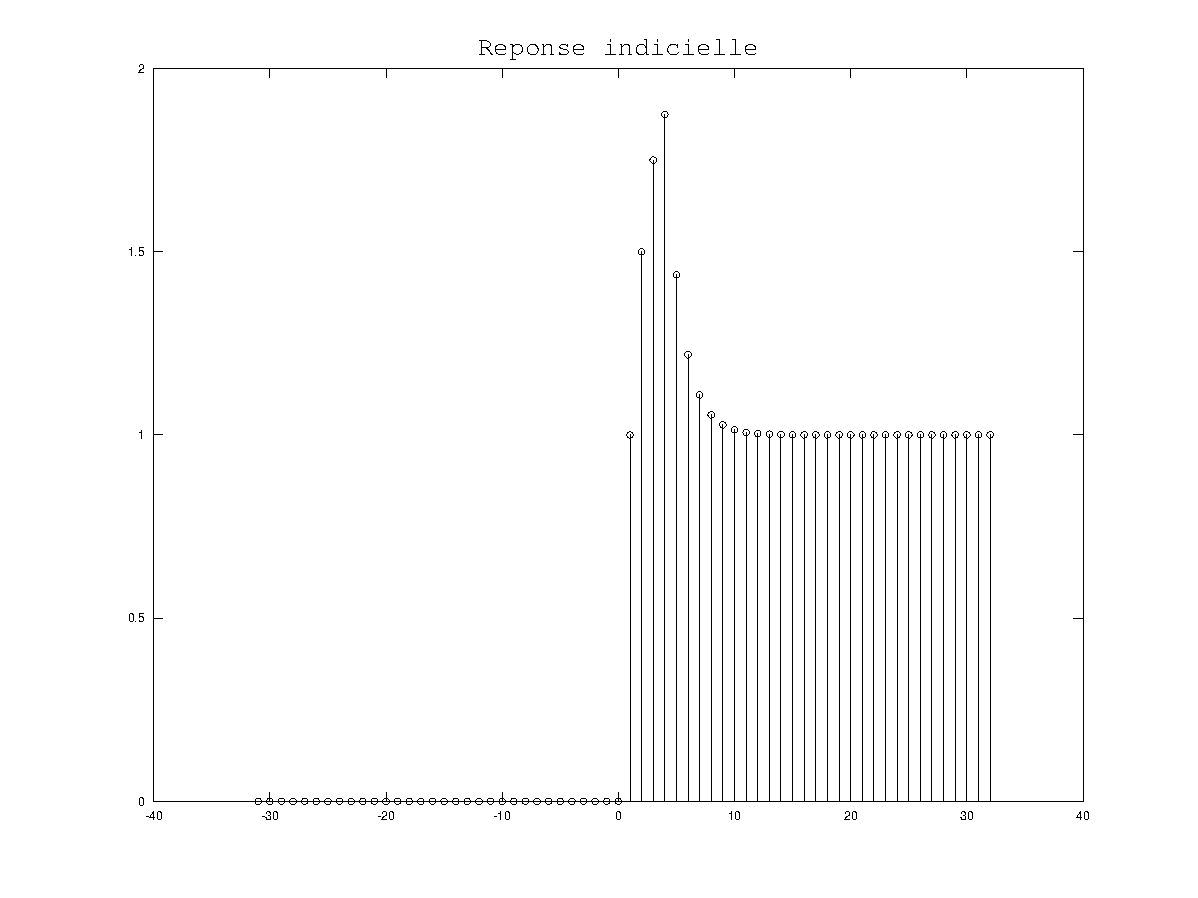
\includegraphics[width=9cm]{resEx3/f5Indice.pdf}
\caption{Réponse indicielle de la fonction $\frac{2z^{-1}-z^{-5}}{2-z^{-1}}$ }
\end{figure}

\subsection{Les zéros et les pôles}
~\\
\begin{figure}[H]
\centering
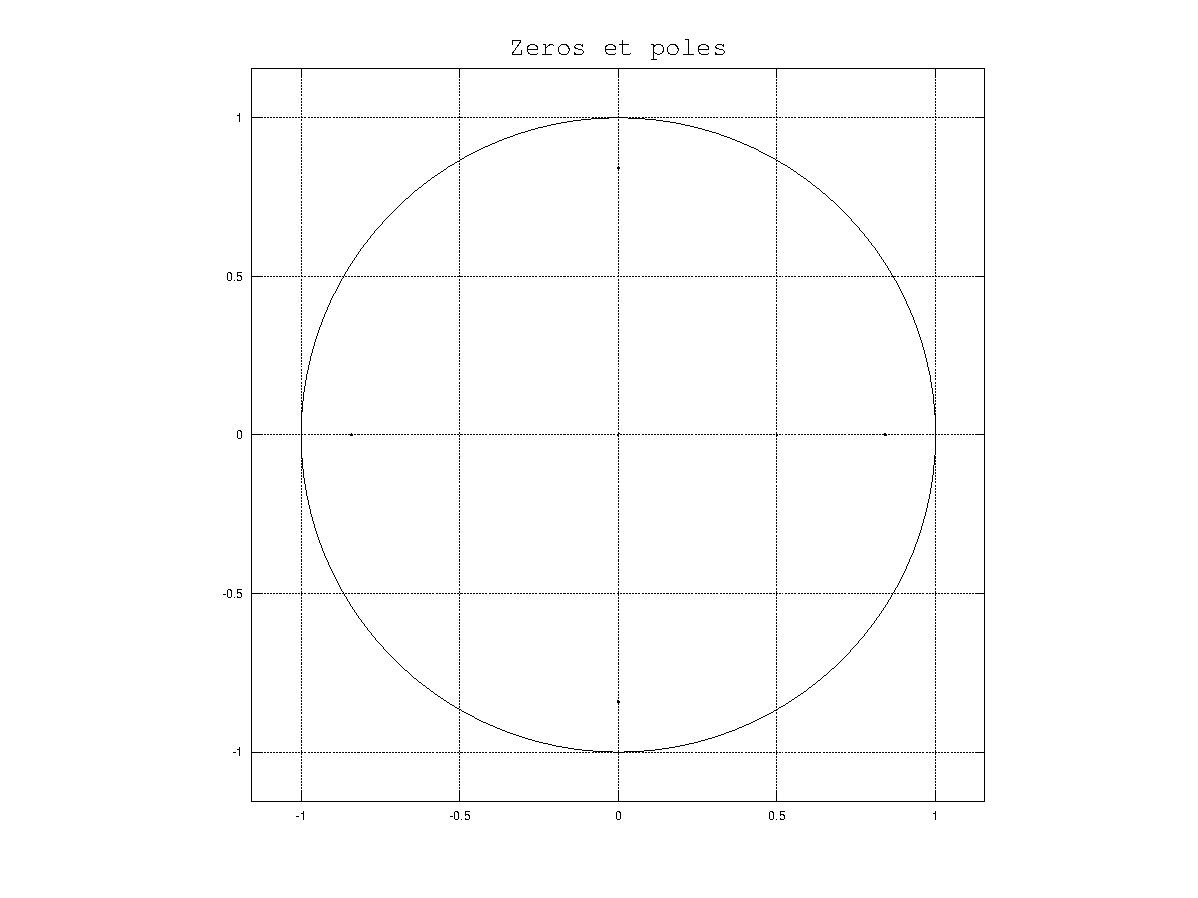
\includegraphics[width=9cm]{resEx3/f5ZP.pdf}
\caption{Les zéros et les pôles de la fonction $\frac{2z^{-1}-z^{-5}}{2-z^{-1}}$ }
\end{figure}


\part{Exercice 4}
Nous créons un filtre passe bas de type Butterworth avec les caractéristiques suivantes:\\
\begin{itemize}
\item Fréquence d'échantillonnage : 8 kHz
\item Fréquence de coupure : 1 kHz
\item Largeur de transition : 200 Hz
\item Ondulation maximale dans la bande passante : 1 dB
\item Atténuation minimaledans la bande coupée : 40 dB
\end{itemize}
~\\
Les trois figures suivantes nous la réponse impulsionnelle, les pôles et les zéros ainsi que la fonction de transfert du filtre que nous avons créé.

\begin{figure}[H]
\centering
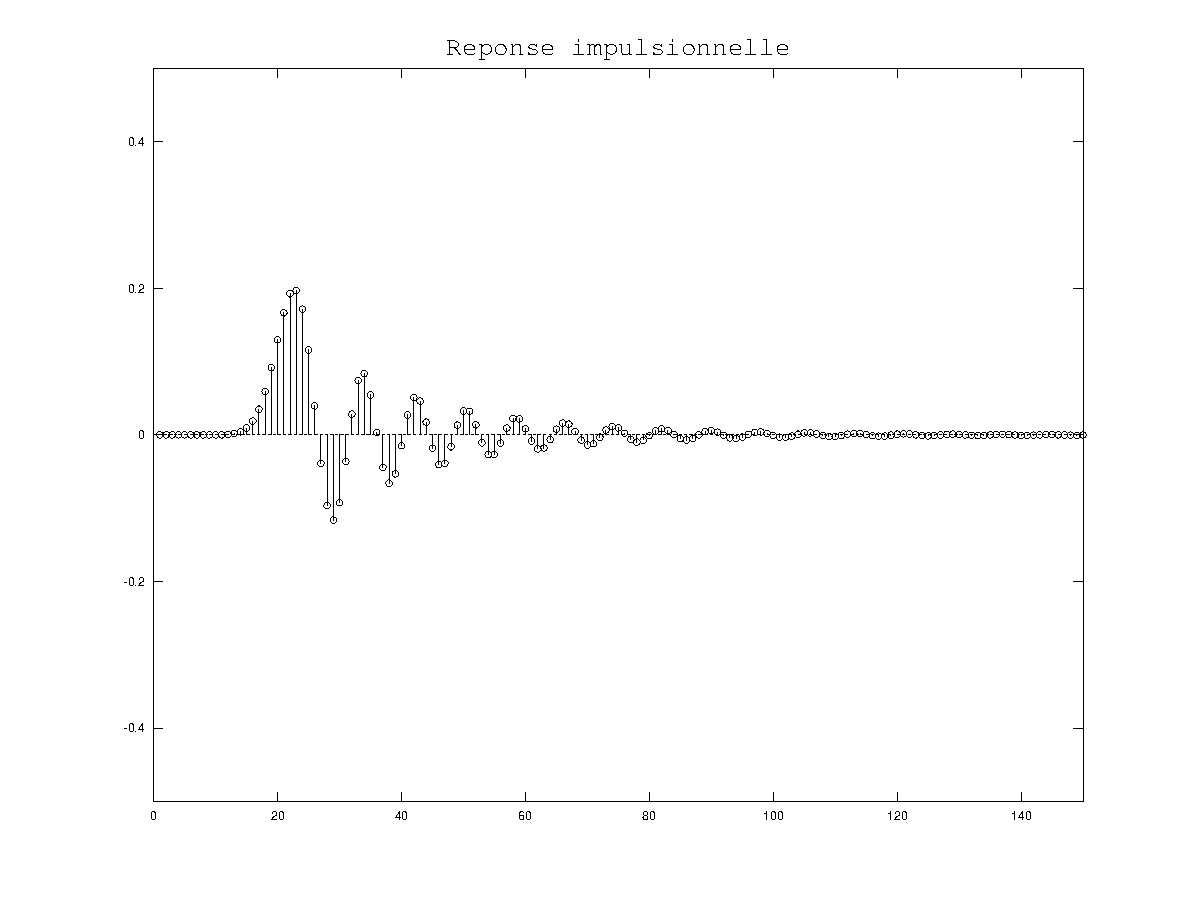
\includegraphics[width=9cm]{resEx4/repImpulsion.pdf}
\caption{Réponse impulsionnelle du filtre de Butterworth}
\end{figure}

\begin{figure}[H]
\centering
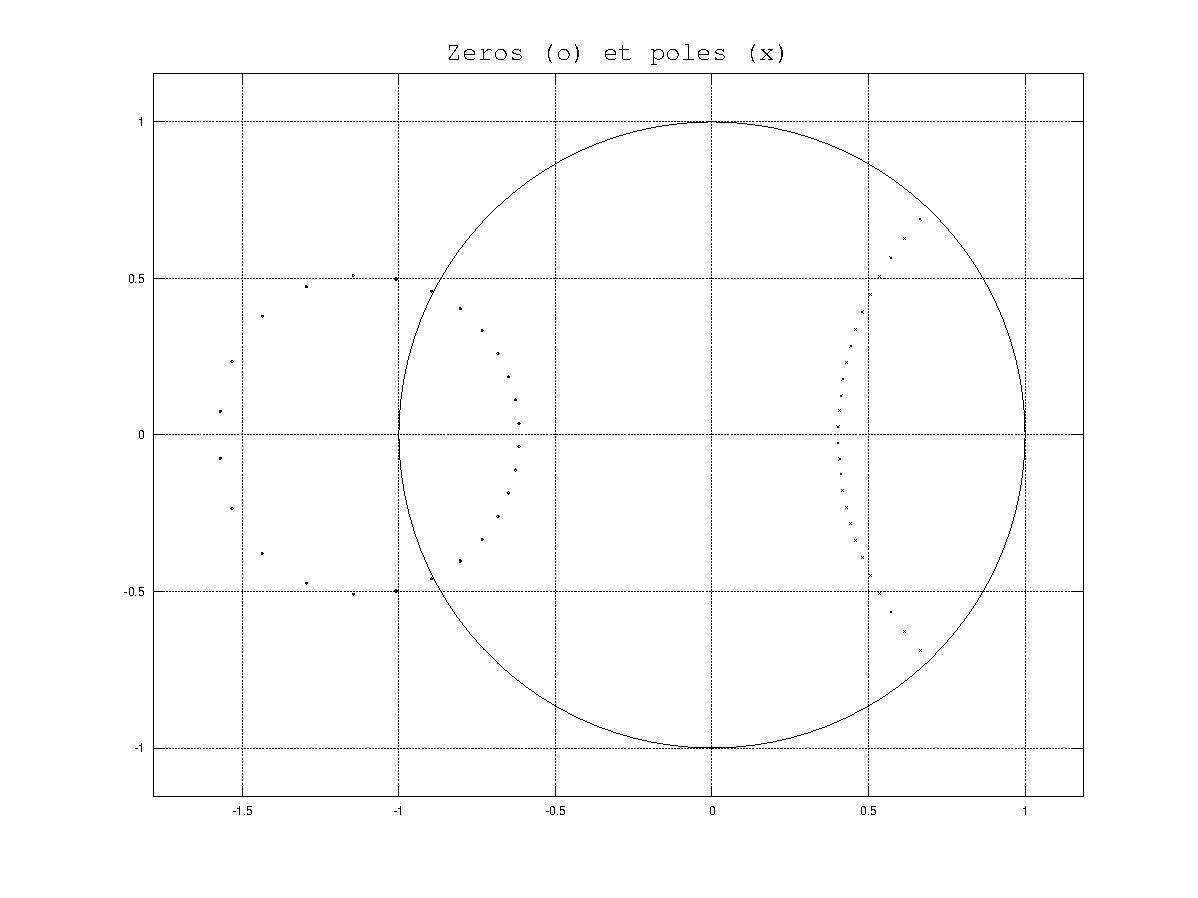
\includegraphics[width=9cm]{resEx4/ZP.pdf}
\caption{Les pôles et les zéros du filtre de Butterworth}
\end{figure}

\begin{figure}[H]
\centering
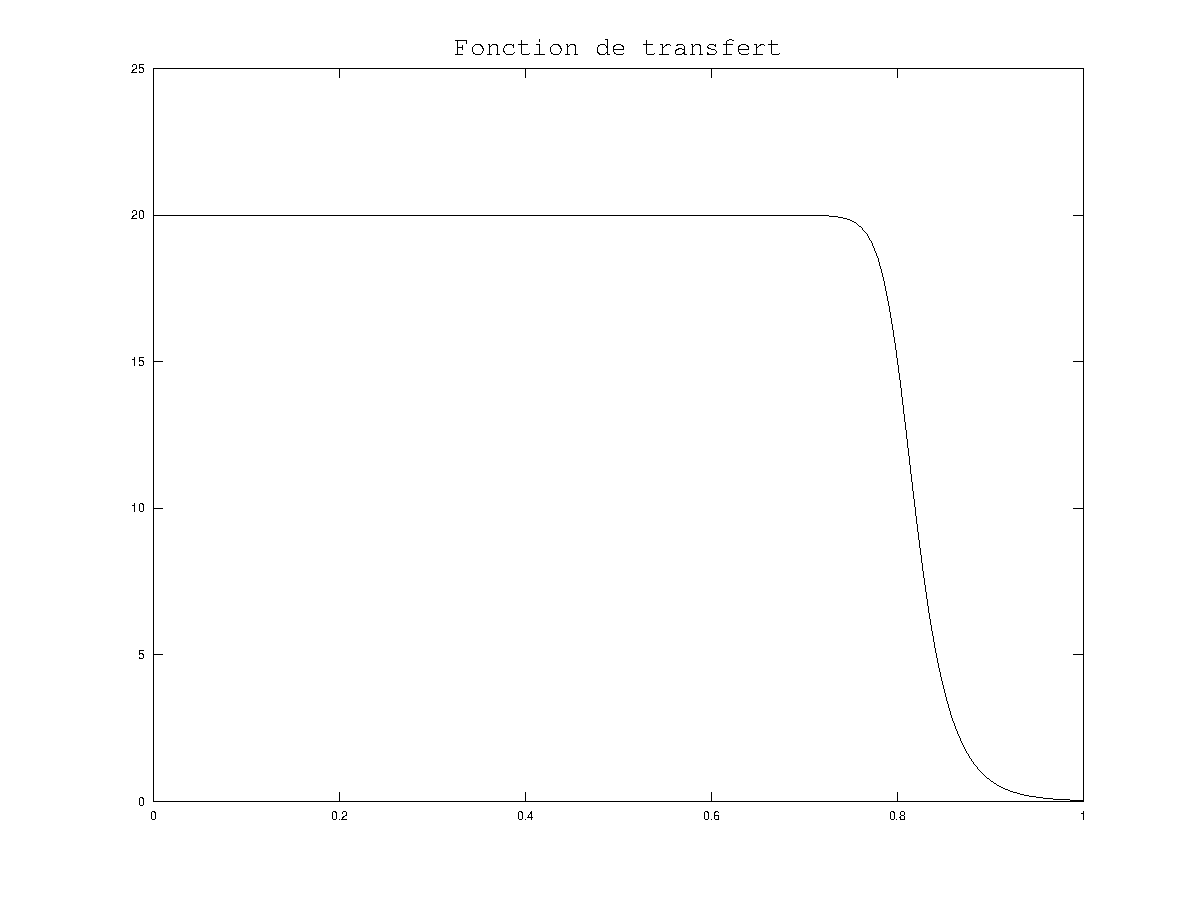
\includegraphics[width=9cm]{resEx4/fctTransfert.pdf}
\caption{Fonction de transfert du filtre de Butterworth}
\end{figure}

Le signal composé de deux sinusoïdes, une de fréquence 800 Hz et l'autre de fréquence 1.4kHz toutes deux échantillonnées à 8 kHz nous donne le signal suivant : 

\begin{figure}[H]
\centering
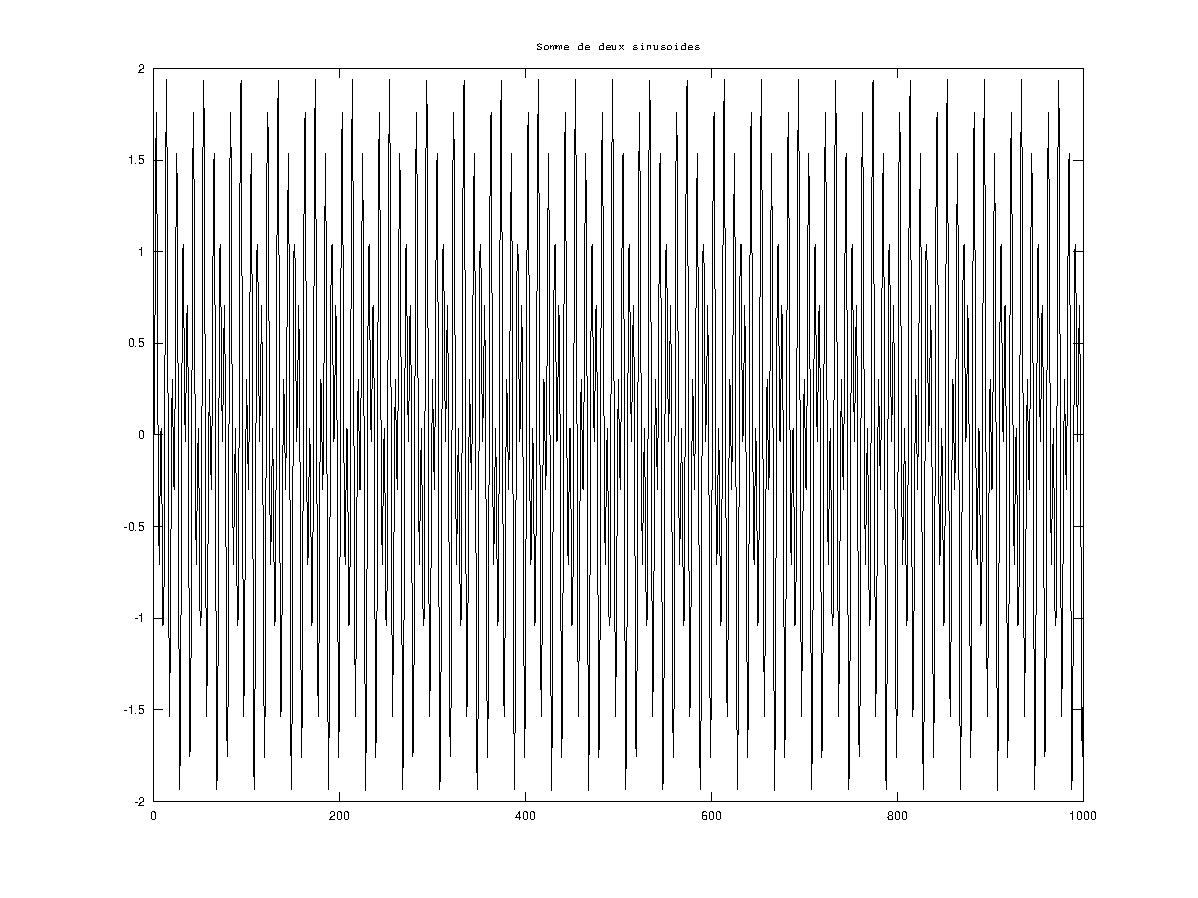
\includegraphics[width=9cm]{resEx4/2sin.pdf}
\caption{Signal formé de deux sinusoïdes}
\end{figure}

Le spectre de ce signal avant filtrage est représenté ci dessous:

\begin{figure}[H]
\centering
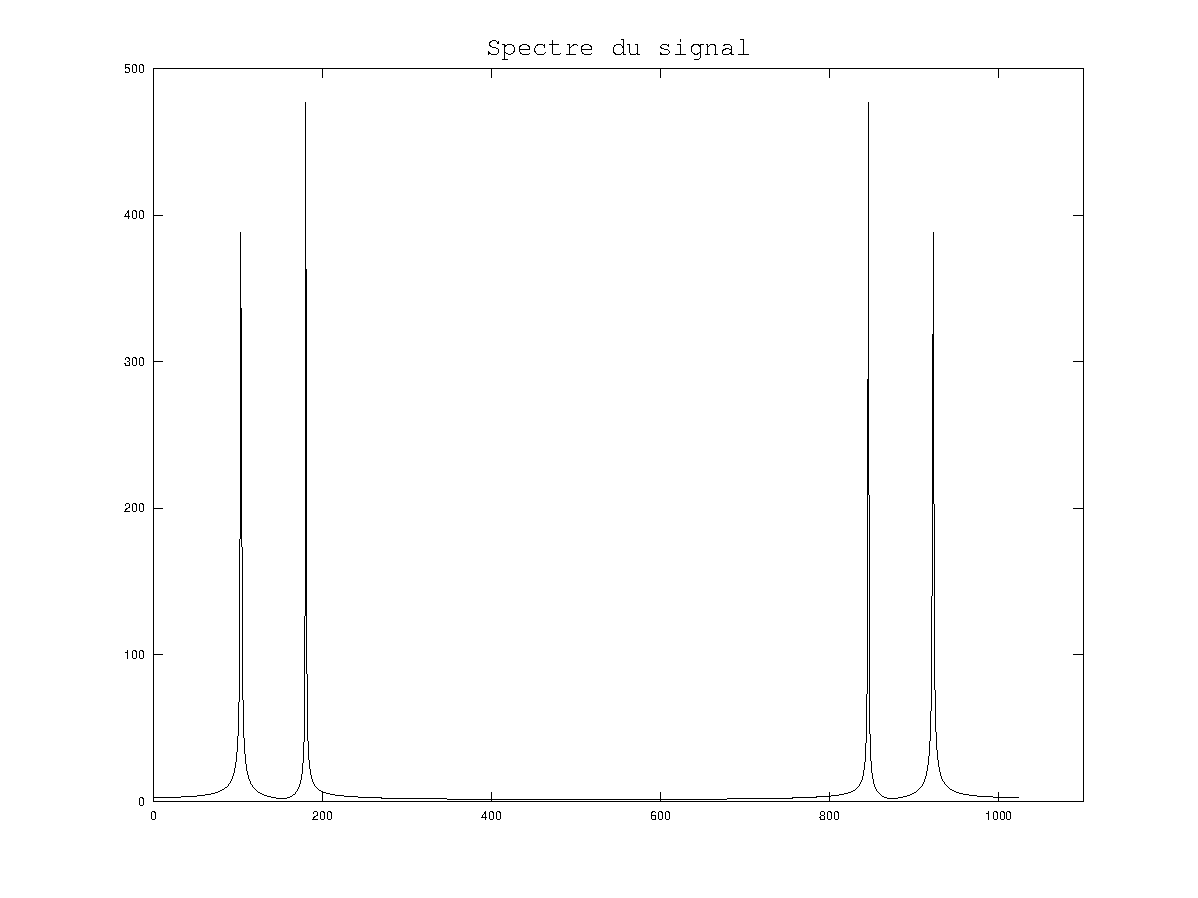
\includegraphics[width=9cm]{resEx4/spectreEntre.pdf}
\caption{Spectre d'entré}
\end{figure}

Une fois que nous lui avons appliqué le filtre nous obtenons:

\begin{figure}[H]
\centering
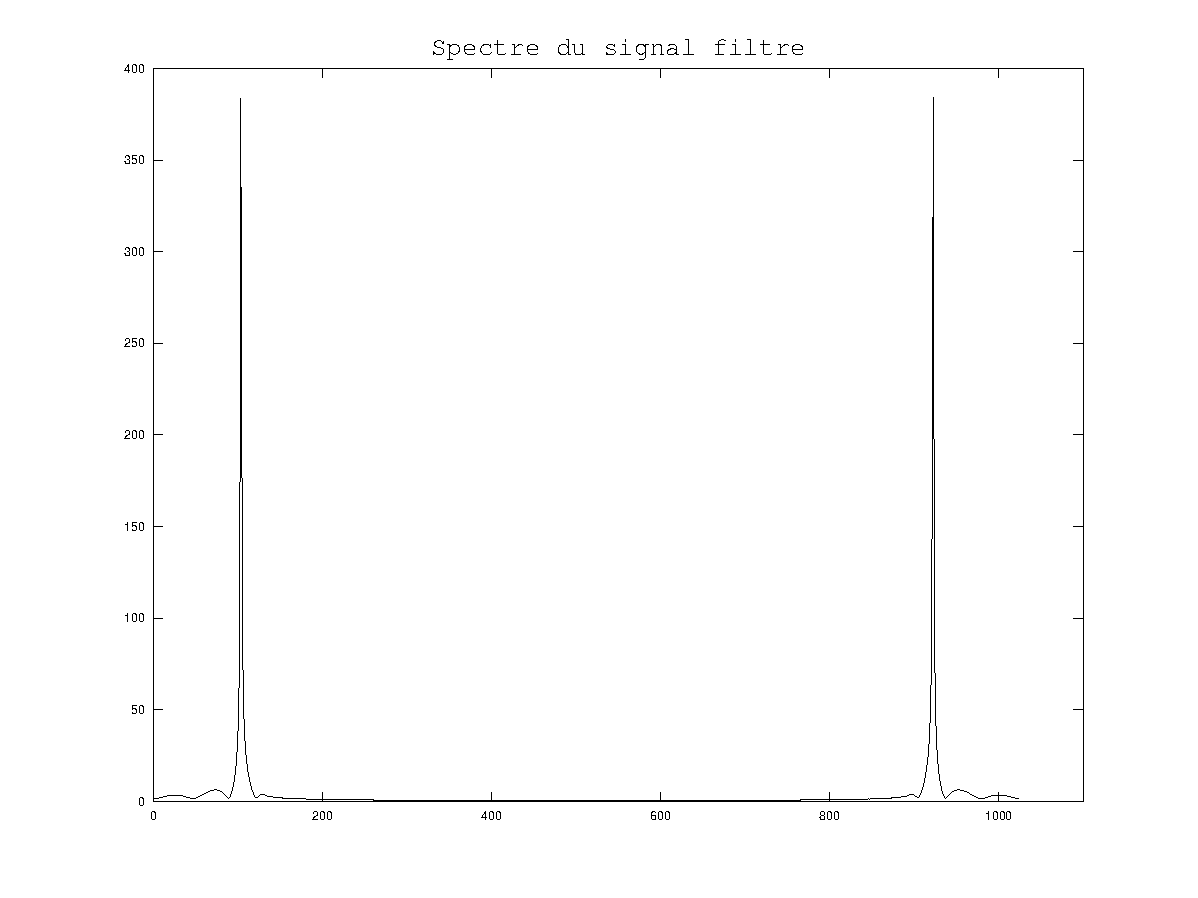
\includegraphics[width=9cm]{resEx4/spectreSortie.pdf}
\caption{Spectre de sortie}
\end{figure}

\part{Exercice 5}
Nous créons une fonction sinus avec les caractéristiques suivantes:\\
\begin{itemize}
\item Fréquence d'échantillonnage : 10 kHz
\item Fréquence du signal : 1 kHz 
\end{itemize}


\begin{figure}[H]
\centering
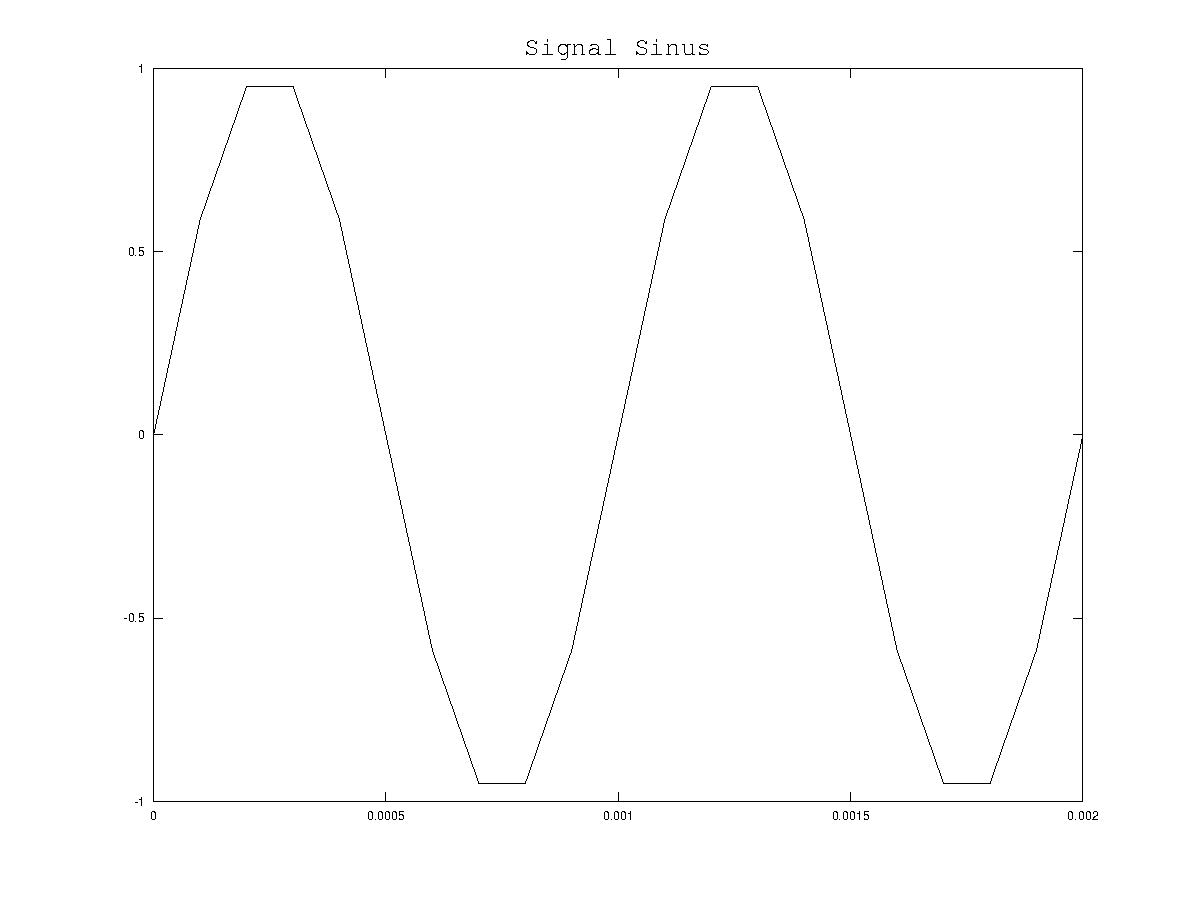
\includegraphics[width=9cm]{resEx5/fig_1_sinus.pdf}
\caption{Signal Sinus : x=$sin(2*pi*fsig*t)$}
\end{figure}


Nous ajoutons un bruit gaussien avec les caractéristiques suivantes:\\
\begin{itemize}
\item Moyenne : null
\item Amplitude : 0.4
\end{itemize}

\begin{figure}[H]
\centering
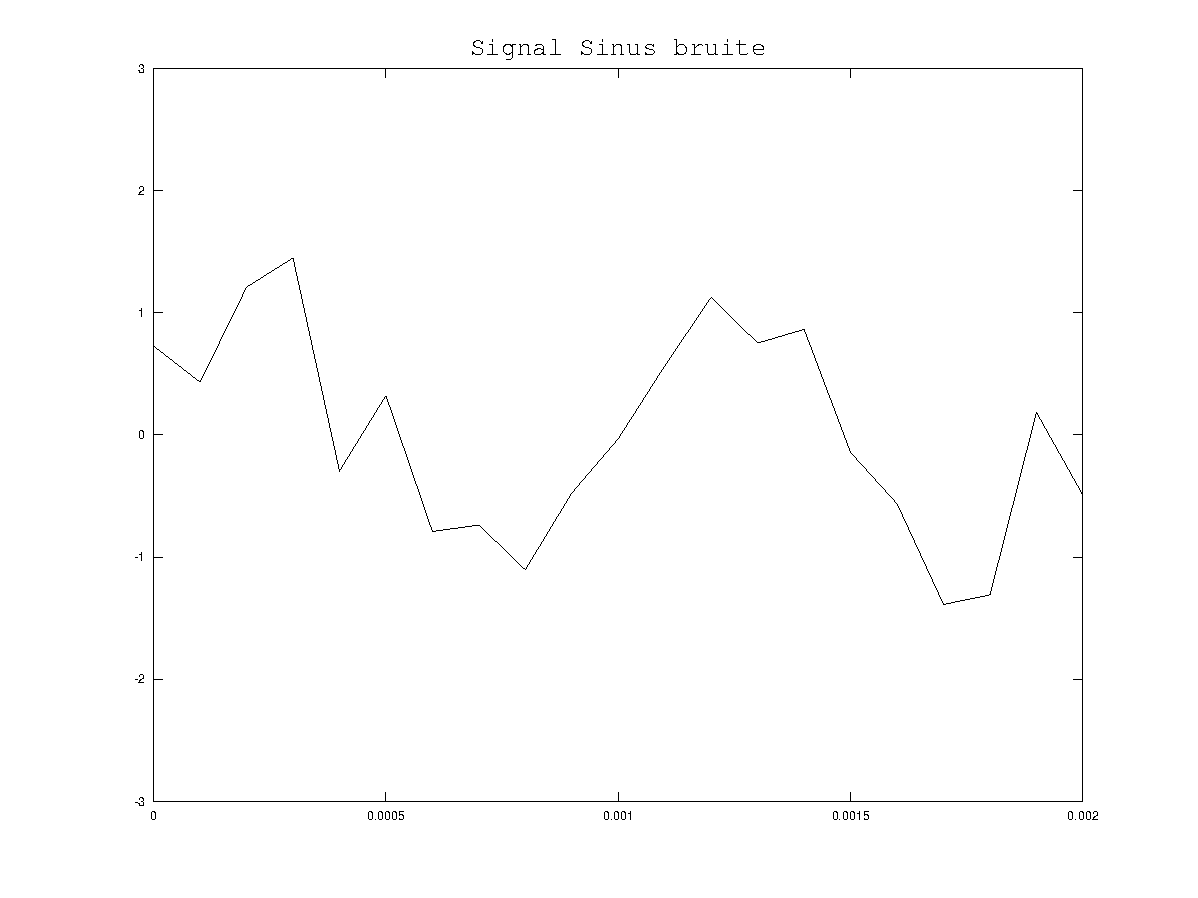
\includegraphics[width=9cm]{resEx5/fig_2_sinusb.pdf}
\caption{Signal Sinus bruité : xB=$ x .+ (moy + ampl*rand(1,N))$}
\end{figure}


Creation d'un filtre passe-bande avec buttord ayant les caractéristiques suivantes:\\
\begin{itemize}
\item Propriété : Ws(1) < Wp(1) < Wp(2) < Ws(2)
\item Ws(1) : 50 
\item Wp(1) : 980 
\item Wp(2) : 1020 
\item Ws(2) : 1450 
\end{itemize}


\begin{figure}[H]
\centering
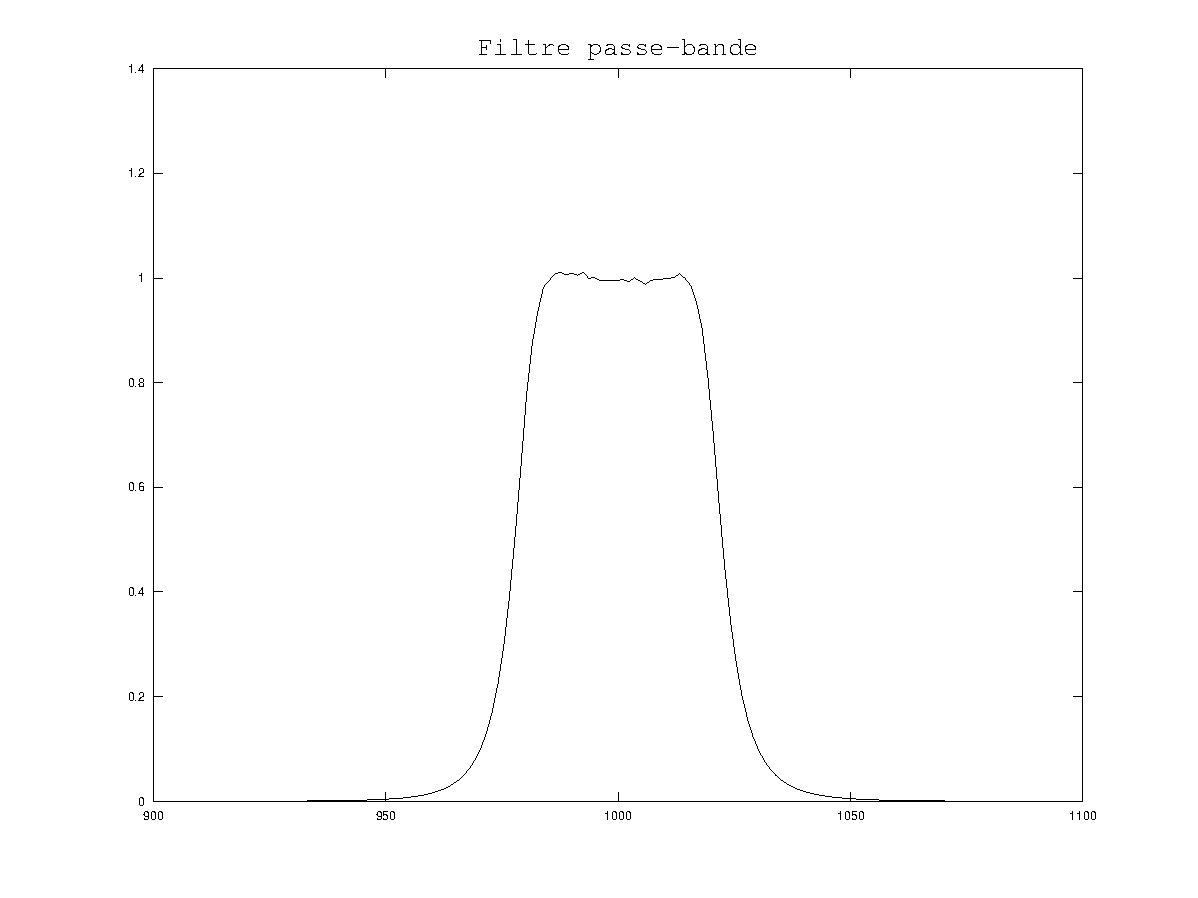
\includegraphics[width=9cm]{resEx5/fig_3_passbande.pdf}
\caption{Filtre Bande Passante visualisé sur l'intervale [900,1100]}
\end{figure}


\begin{figure}[H]
\centering
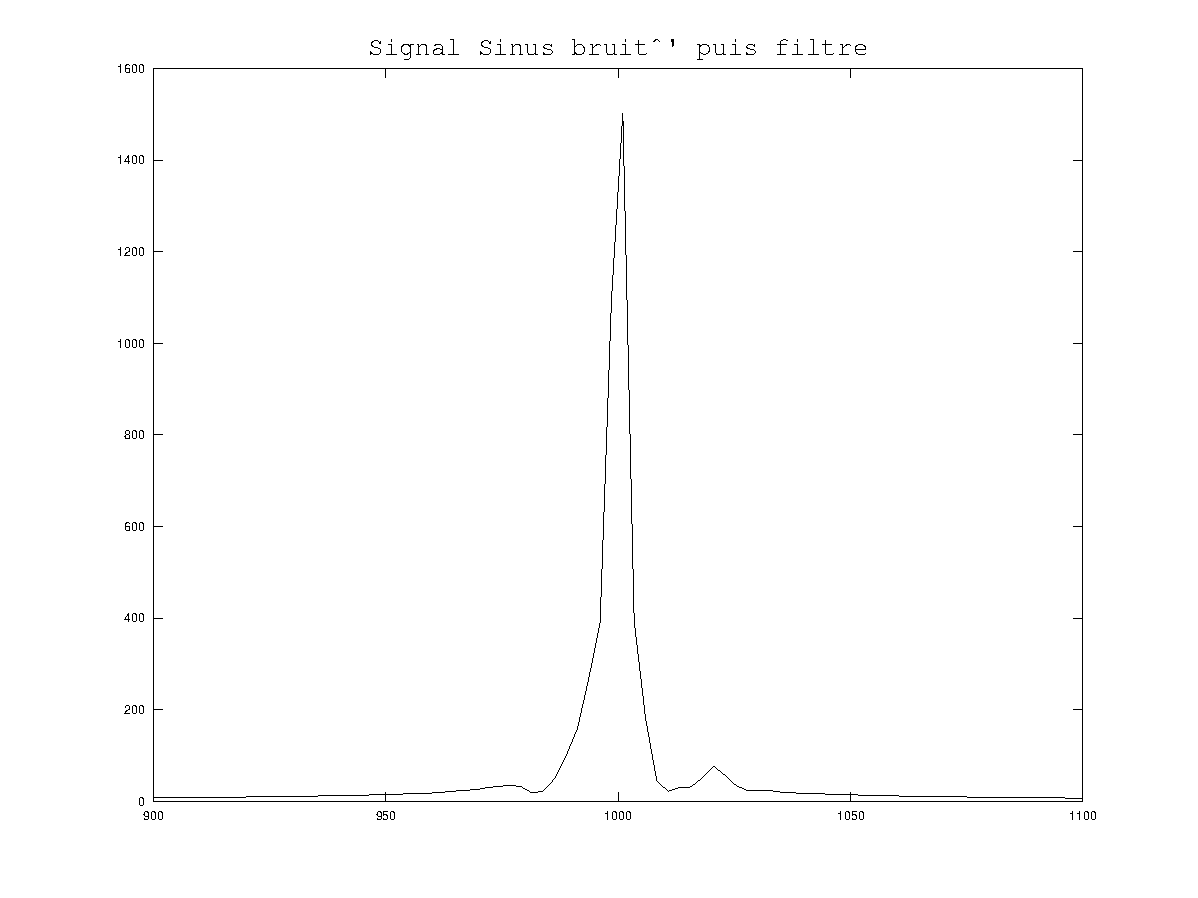
\includegraphics[width=9cm]{resEx5/fig_5_sinus-b.pdf}
\caption{Application du Filtre Bande Passante}
\end{figure}


\begin{figure}[H]
\centering
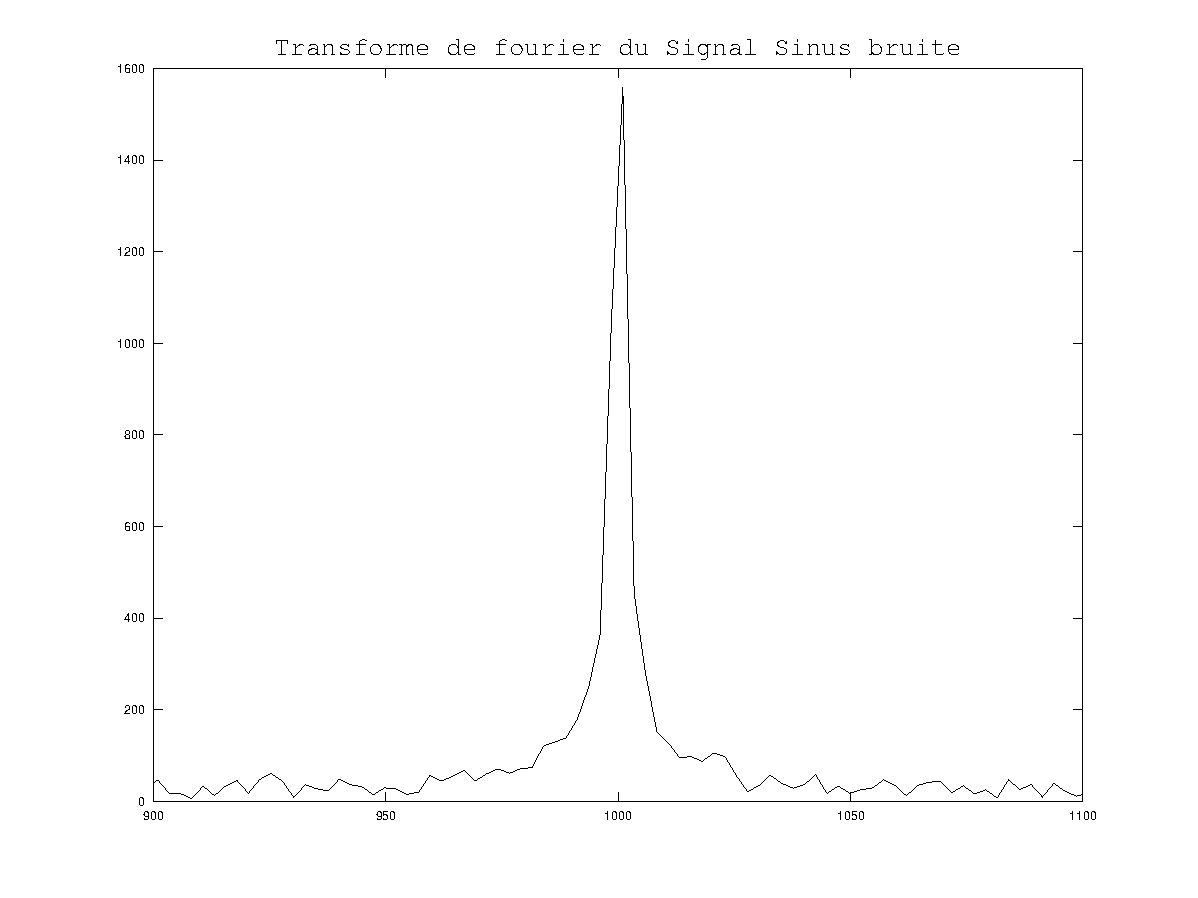
\includegraphics[width=9cm]{resEx5/fig_4_fftsinusb.pdf}
\caption{Transforme de fourier du Signal Sinus bruite}
\end{figure}


En comparant la courbe de la transformation de fourier du signal bruité FIG 42 et la courbe du signal bruité filtré FIG 41, nous remarquons autour de la frequence 1KHz ( le pic de la courbe ) que le bruit discorde moins la courbe et à donc été atténué .



\part{Exercice 6}


\begin{figure}[H]
\centering
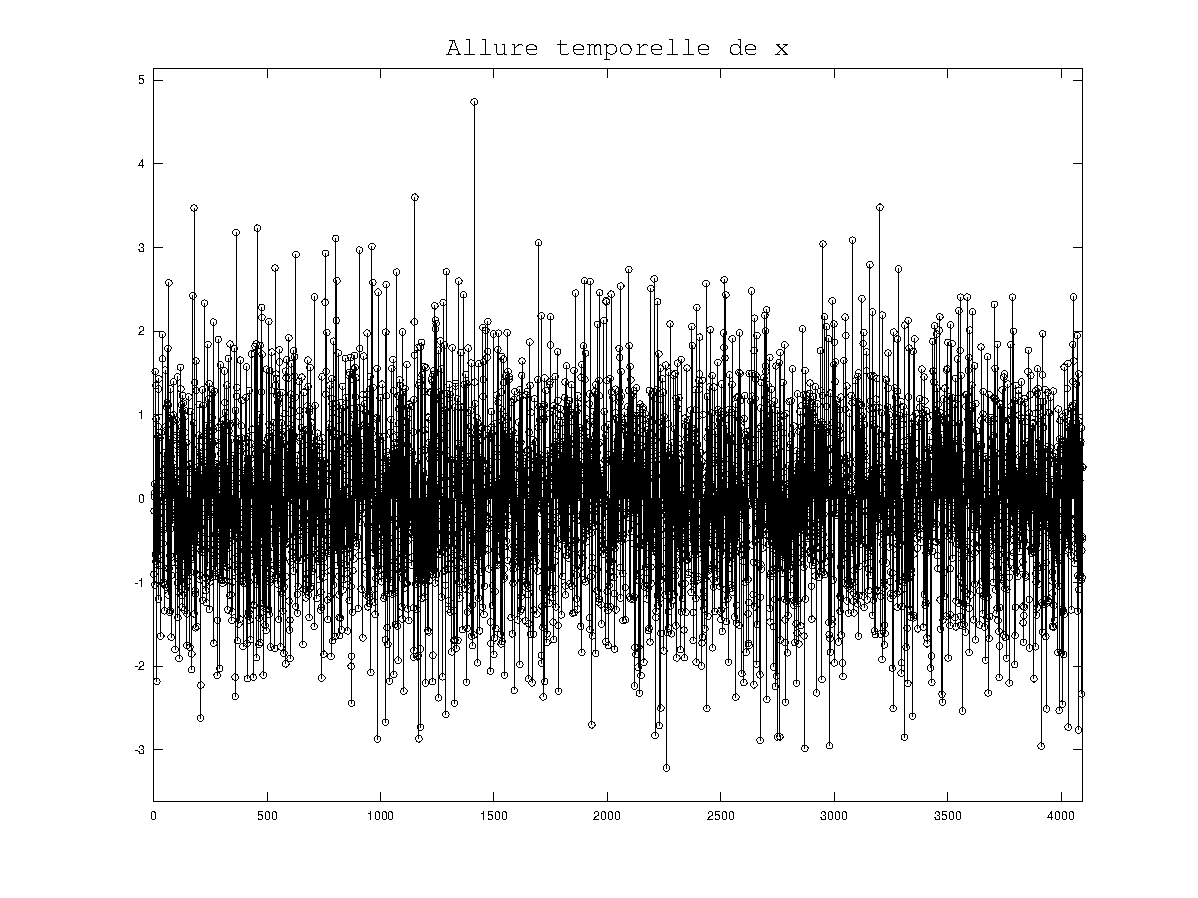
\includegraphics[width=9cm]{resEx6/fig_1.pdf}
\caption{Allure temporelle de x}
\end{figure}


\begin{figure}[H]
\centering
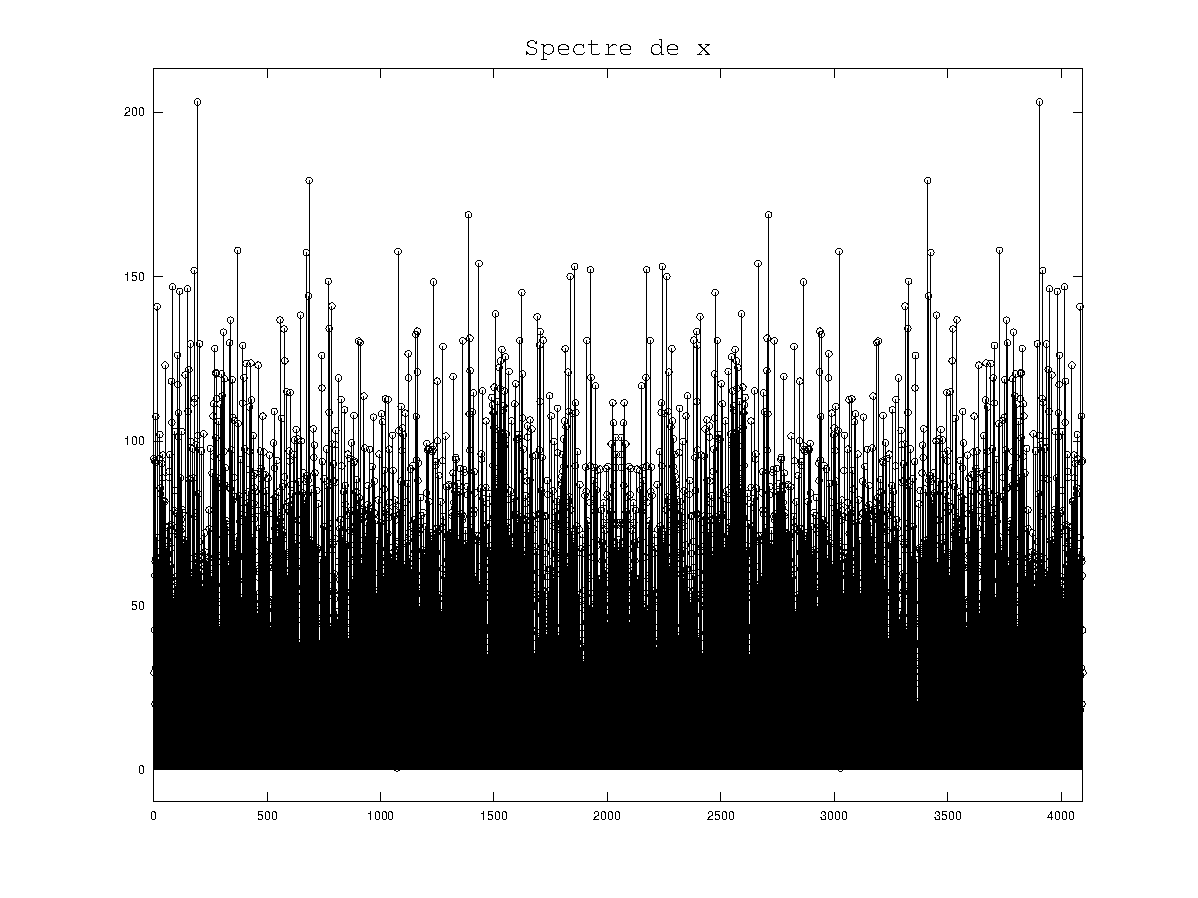
\includegraphics[width=9cm]{resEx6/fig_2.pdf}
\caption{Spectre de x}
\end{figure}


\begin{figure}[H]
\centering
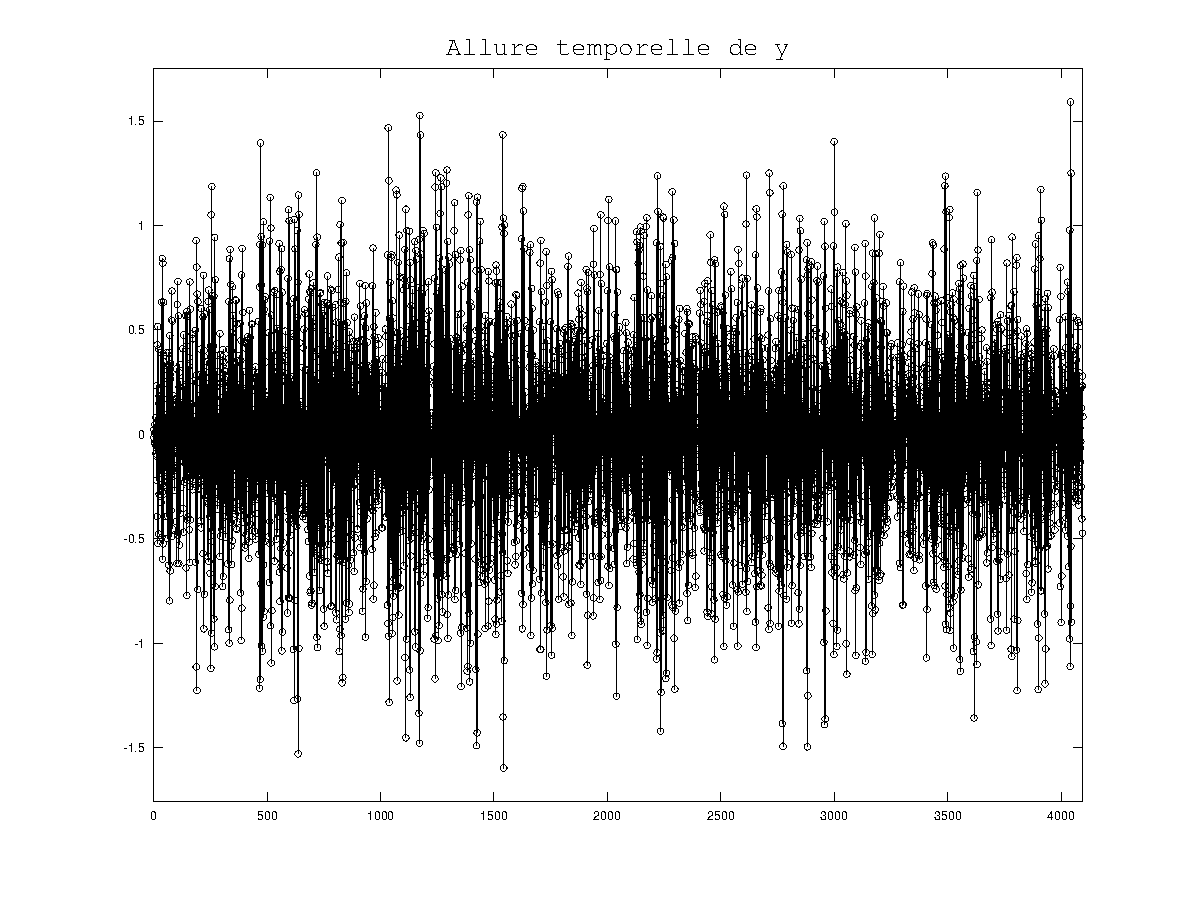
\includegraphics[width=9cm]{resEx6/fig_3.pdf}
\caption{Allure temporelle de y}
\end{figure}


\begin{figure}[H]
\centering
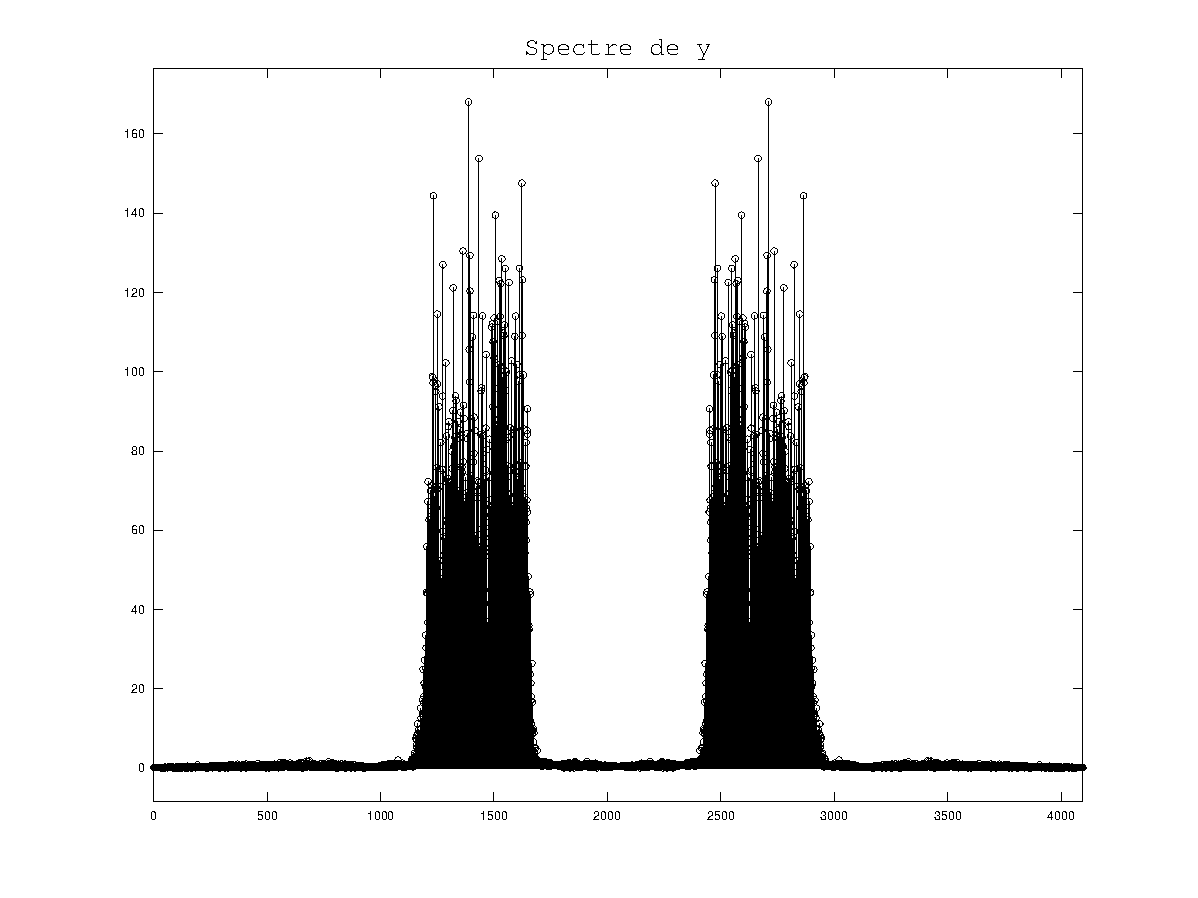
\includegraphics[width=9cm]{resEx6/fig_4.pdf}
\caption{Spectre de y}
\end{figure}


Les caractéristiques du signal x:\\
\begin{itemize}
\item Moyenne : 0.02
\item Ecart type : 1.01
\item Variance : 1.02
\end{itemize}


\begin{figure}[H]
\centering
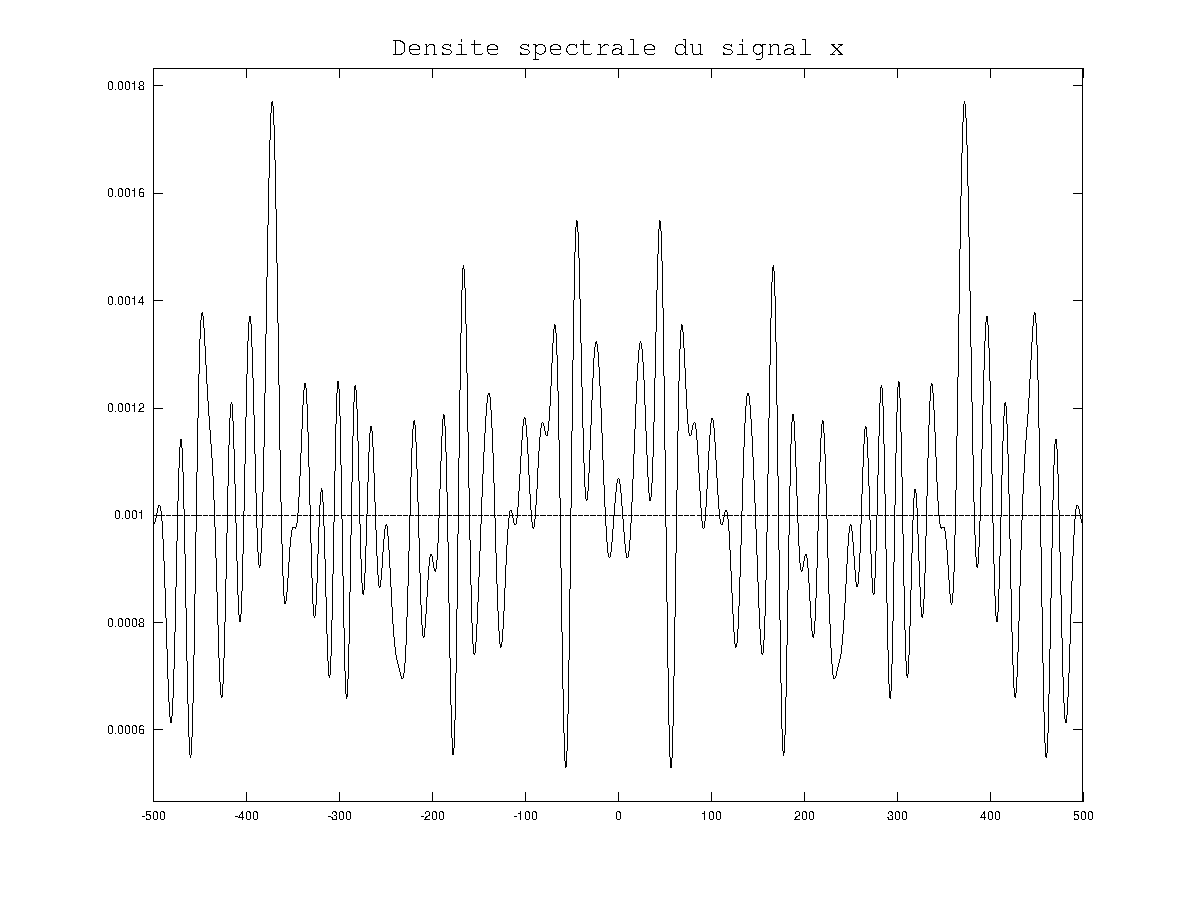
\includegraphics[width=9cm]{resEx6/fig_5.pdf}
\caption{Densite spectrale du signal x}
\end{figure}


\begin{figure}[H]
\centering
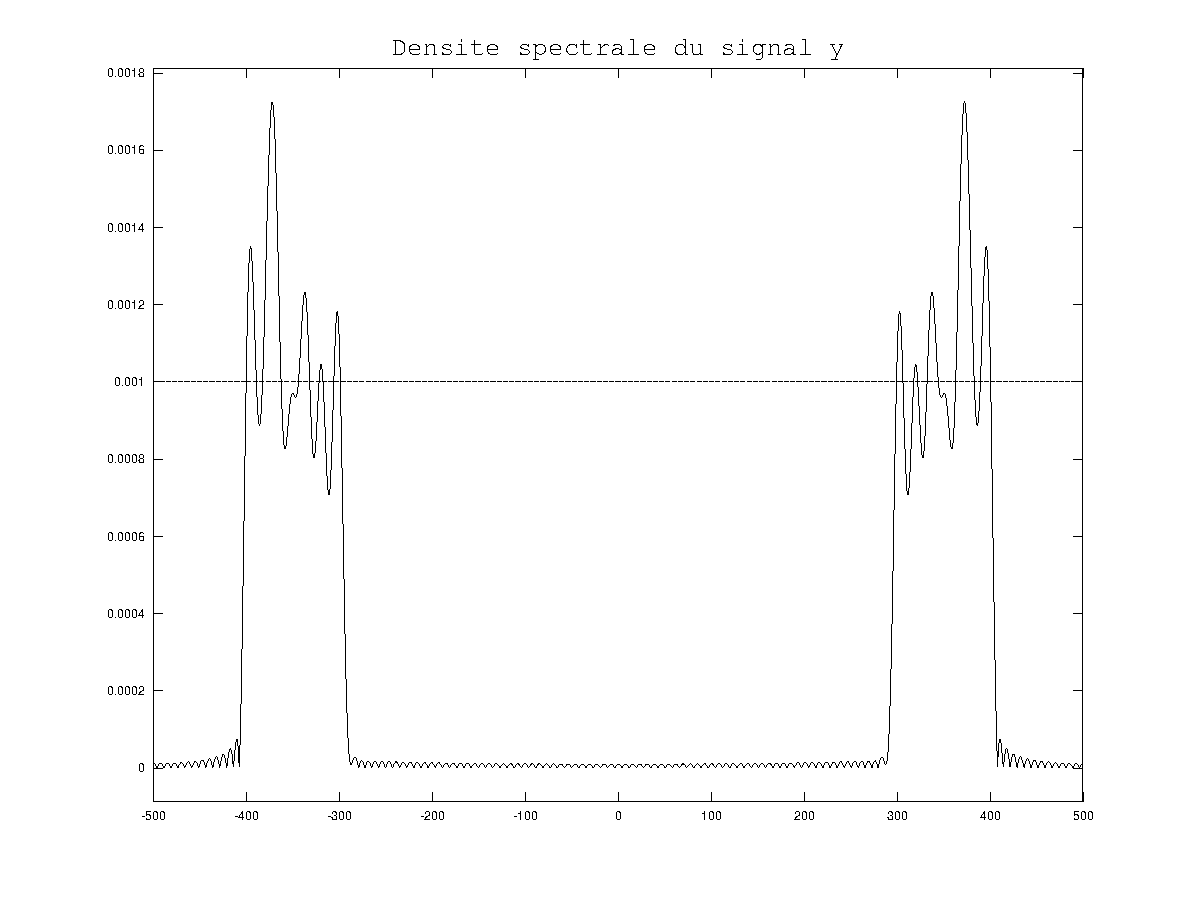
\includegraphics[width=9cm]{resEx6/fig_6.pdf}
\caption{Densite spectrale du signal y}
\end{figure}



Nous déduisons l’allure de la fonction de transfert harmonique du filtre grâce à la racine carré de la densité spectral en sortie / densité spectrale en entrée.

\begin{figure}[H]
\centering
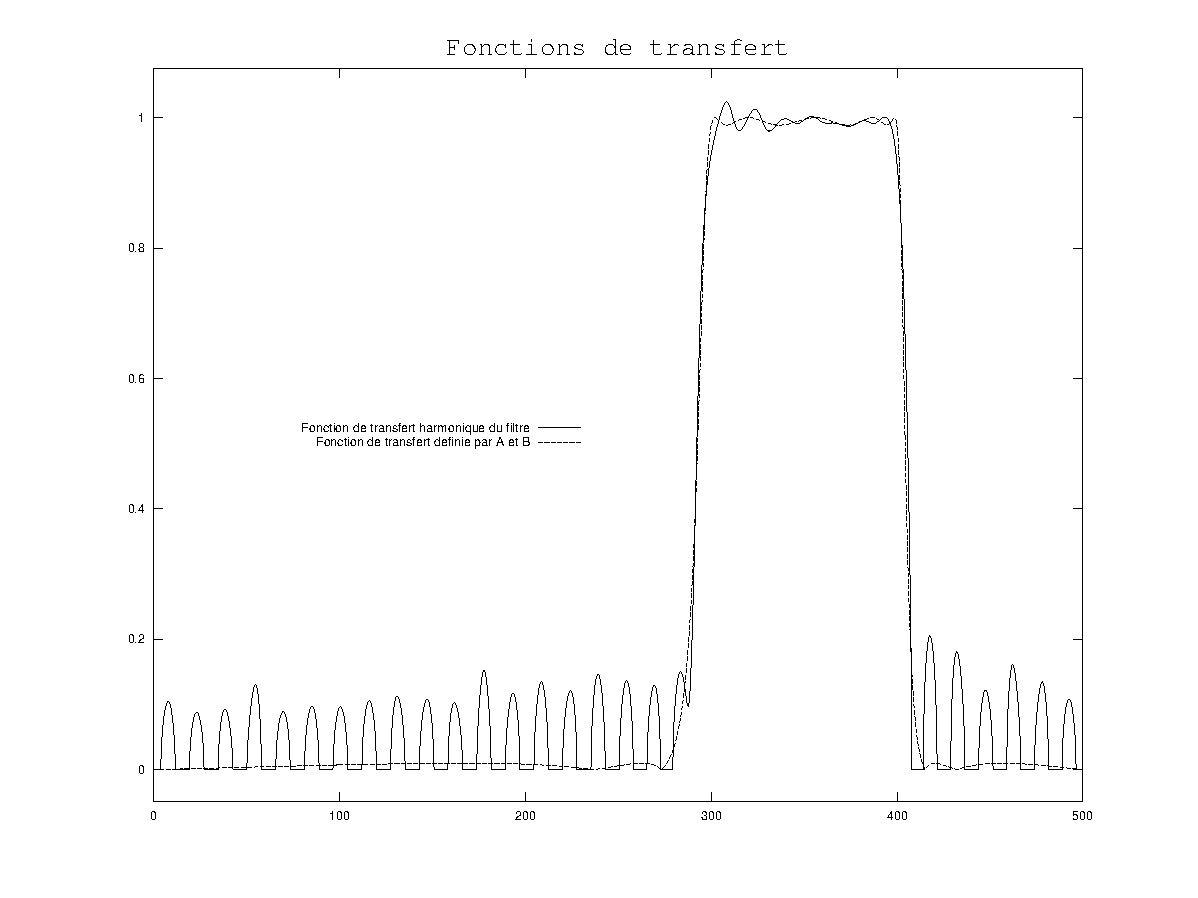
\includegraphics[width=9cm]{resEx6/fig_7.pdf}
\caption{Comparaison des Fonctions de transfert.}
\end{figure}



\end{document} % fin du document
%EOF

